\RequirePackage[ngerman=ngerman-x-latest]{hyphsubst}
\documentclass[english,ngerman]{tudscrreprt}
\usepackage{babel}
\usepackage{selinput}
\SelectInputMappings{adieresis={ä},germandbls={ß}}
\usepackage[T1]{fontenc}
\usepackage{fixltx2e}
\usepackage{scrhack}
\usepackage{tudscrsupervisor}
\usepackage{xcolor}
\usepackage{gensymb}

%%%
% Glossar
%
\AfterPackage*{hyperref}{%
	\usepackage[%
		automake,% Alphabetische Sortierung, da xindy aktiv, kein makeindex benötigt
		% mit Tex Live einfach verwendbar
		xindy={language=german-din}, % Alphabetische Sortierung nach UTF-8 und Duden oder DIN.
		acronym,% Abkürzungen
		symbols,% Formelzeichen
		%nomain,% kein Glossar
		translate=babel,% Überschriften der Glossare in der Dokumentsprache gesetzt
		nogroupskip,% automatischer Abstand zwischen den Einträgen zur Gruppierung innerhalb eines Glossars entfernen
		toc,% fügt die Verzeichnisse dem Inhaltsverzeichnis hinzu
		section=chapter,% bestimmt die Gliederungsebene der Überschrift
	]{glossaries}
	\makeglossaries
	
\newglossarystyle{acrotabu}{%
	\renewenvironment{theglossary}{%
		\begin{tabu}spread 0pt{@{}lX<{\strut}l@{}}%
	}{%
		\end{tabu}\par\bigskip%
	}%
	\renewcommand*{\glossaryheader}{}%
	\renewcommand*{\glsgroupheading}[1]{}%
	\renewcommand*{\glsgroupskip}{}%
	\renewcommand*{\glossentry}[2]{%
		\glsentryitem{##1}% Entry number if required
		\glstarget{##1}{\sffamily\bfseries\glossentryname{##1}} &
		\glsentrydesc{##1} &
		##2\tabularnewline
	}
}

\newcommand*{\newsymbol}[5][]{%
	\newglossaryentry{#2}{%
		type=symbols,%
		description={},%
		name={#3},%
		symbol={\ensuremath{#4}},%
		user1={\ensuremath{\mathrm{#5}}},%
		sort={#2},%
		#1%
	}%
}

\defglsentryfmt[symbols]{%
	\ifmmode%
	\glssymbol{\glslabel}%
	\else%
	\glsgenentryfmt~\glsentrysymbol{\glslabel}%
	\fi%
}
\newglossarystyle{symblongtabu}{%
	\renewenvironment{theglossary}{%
		\begin{longtabu}spread 0pt[l]{ccX<{\strut}l}%
		}{%
		\end{longtabu}%
	}%
	\renewcommand*{\glossaryheader}{%
		\toprule
		\bfseries Symbol & \bfseries Einheit &
		\bfseries Name & \bfseries Seite(n)
		\tabularnewline\midrule\endhead%
		\bottomrule\endfoot%
	}%
	\renewcommand*{\glsgroupheading}[1]{}%
	\renewcommand*{\glsgroupskip}{}%
	\renewcommand*{\glossentry}[2]{%
		\glsentryitem{##1}% Entry number if required
		\glstarget{##1}{\glossentrysymbol{##1}} &
		\glsentryuseri{##1} &
		\glossentryname{##1} &
		##2\tabularnewline%
	}%
}
}% Ende von AfterPackage*

%%%
% Zitate
%
\usepackage{csquotes}
\usepackage[backend=biber,style=alphabetic]{biblatex}
\addbibresource{bib/MMandCountourTrees.bib}
\addbibresource{bib/Polyeder.bib}

%%%
% Caption
%
\usepackage{caption}
\captionsetup{font=sf,labelfont=bf,labelsep=space}
\usepackage{floatrow}
\floatsetup{font=sf}
\floatsetup[table]{style=plaintop}
\captionsetup{singlelinecheck=off,format=hang,justification=raggedright}
\DeclareCaptionSubType[alph]{figure}
\DeclareCaptionSubType[alph]{table}
\captionsetup[subfloat]{labelformat=brace,list=off}

%%%
% Tabellen
%
\usepackage{booktabs} % Linien für Tabellen.
\usepackage{array} % Definitionen für Spalten.
\usepackage{tabularx} % Tabellen mit gleicher Spaltenbreite.
\usepackage{tabulary}
\usepackage{tabu}


%%%
% Index
%
\usepackage{imakeidx}
\indexsetup{%
	level=\chapter*,
	noclearpage, firstpagestyle=headings, headers={\indexname}{\indexname},
	othercode={\renewcommand*\subitem{\@idxitem\hspace*{15\p@}}}
}\makeindex

%%%
% Bilder
%
\usepackage{graphicx}
\graphicspath{ {./media/} }

%%%
% Quellcode
%
\usepackage{listings}
% UTF8
\lstset{%
	inputencoding = utf8,
	extendedchars = true, % lets you use non-ASCII characters; for 8-bits encodings only, does not work with UTF-8
	literate=%
	{ä}{{\"a}}1 {ö}{{\"o}}1 {ü}{{\"u}}1
	{Ä}{{\"A}}1 {Ö}{{\"O}}1 {Ü}{{\"U}}1
	{~}{{\textasciitilde}}1 {ß}{{\ss}}1
}
\definecolor{dkgreen}{rgb}{0,0.6,0}
\definecolor{mygray}{rgb}{0.5,0.5,0.5}
\definecolor{mymauve}{rgb}{0.58,0,0.82}
\lstset{ %
	backgroundcolor=\color{white},   % choose the background color; you must add \usepackage{color} or \usepackage{xcolor}
	basicstyle=\footnotesize,        % the size of the fonts that are used for the code
	breakatwhitespace=false,         % sets if automatic breaks should only happen at whitespace
	breaklines=true,                 % sets automatic line breaking
	captionpos=b,                    % sets the caption-position to bottom
	commentstyle=\color{dkgreen},    % comment style
	deletekeywords={...},            % if you want to delete keywords from the given language
	escapeinside={\%*}{*)},          % if you want to add LaTeX within your code
	frame=single,                    % adds a frame around the code
	keepspaces=true,                 % keeps spaces in text, useful for keeping indentation of code (possibly needs columns=flexible)
	keywordstyle=\color{blue},       % keyword style
	language=Octave,                 % the language of the code
	morekeywords={*,...},            % if you want to add more keywords to the set
	numbers=left,                    % where to put the line-numbers; possible values are (none, left, right)
	numbersep=5pt,                   % how far the line-numbers are from the code
	numberstyle=\tiny\color{mygray}, % the style that is used for the line-numbers
	rulecolor=\color{black},         % if not set, the frame-color may be changed on line-breaks within not-black text (e.g. comments (green here))
	showspaces=false,                % show spaces everywhere adding particular underscores; it overrides 'showstringspaces'
	showstringspaces=false,          % underline spaces within strings only
	showtabs=false,                  % show tabs within strings adding particular underscores
	stepnumber=2,                    % the step between two line-numbers. If it's 1, each line will be numbered
	stringstyle=\color{mymauve},     % string literal style
	tabsize=2,                       % sets default tabsize to 2 spaces
	title=\lstname                   % show the filename of files included with \lstinputlisting; also try caption instead of title
}

%%%
% Links
%
\usepackage{hyperref} % Möglichst am Ende stehen, da es viele Befehle neu definiert.
\hypersetup{
	colorlinks   = true, %Colours links instead of ugly boxes
	urlcolor     = HKS41!70, %Colour for external hyperlinks
	linkcolor    = HKS44!70, %Colour of internal links
	citecolor    = HKS33!80 %Colour of citations
}

\usepackage{quoting}

\usepackage[babel]{microtype}

\usepackage{xfrac}

%%%
% Aufzählungen
%
\usepackage{enumitem}
\setlist[itemize]{noitemsep}
\setlist[description]{noitemsep}

\usepackage{isodate}

\usepackage{ellipsis}
\let\ellipsispunctuation\relax

\usepackage{amssymb} % Muss nach hyperref kommen, sonst Fehler "\newsymbol already defined". Alternative: http://tex.stackexchange.com/questions/73684/are-there-any-situtations-where-it-is-better-to-load-a-package-after-other-code

\usepackage{tikz}
\usetikzlibrary{arrows,positioning,scopes,trees}
%%%
% Index
%
\newcommand{\CFD}{\gls{cfd}\index{CFD-Algorithmus}}
\newcommand{\SECC}{\gls{secc}\index{SECC-Algorithmus}}

%Allgemein
\newcommand{\tool}[1]{\textit{#1}\index{#1}} %und libs. Wg vieler Abkürzungen evtl ins Glossar! (z.B. ANN, OpenMP, PPL)
\newcommand{\tools}[2]{\textit{#1}\index{#2}}
\newcommand{\propername}[1]{\textit{#1}\index{#1}} % Allgemein.
\newcommand{\propernames}[2]{\textit{#1}\index{#2}} % Allgemein.
\newcommand{\SEPlugin}[1]{\textit{#1}\index{#1}} % Programmaufbau, evtl in Glossar umwandeln!
\newcommand{\SEPlugins}[2]{\textit{#1}\index{#2}} % Programmaufbau.

%Visualisierung
\newcommand{\visattr}[1]{\textit{#1}\index{#1}}
\newcommand{\visattrs}[2]{\textit{#1}\index{#2}}
\newcommand{\vis}[1]{\textit{#1}\index{#1}} %Visuelles
\newcommand{\viss}[2]{\textit{#1}\index{#2}} %Visuelles
\newcommand{\dataparam}[1]{\textit{#1}\index{#1}}
\newcommand{\dataparams}[2]{\textit{#1}\index{#2}}

% Berechnung
\newcommand{\contour}[1]{\textit{#1}\index{#1}}
\newcommand{\contours}[2]{\textit{#1}\index{#2}}
\newcommand{\SECterm}[1]{\textit{#1}\index{#1}}
\newcommand{\SECterms}[2]{\textit{#1}\index{#2}}
\newcommand{\CFDterm}[1]{\textit{#1}\index{#1}}
\newcommand{\CFDterms}[2]{\textit{#1}\index{#2}}

%%%
% Auszeichnungen
%
\newcommand{\wichtig}[1]{\textit{#1}}
\newcommand{\mrkg}[1]{\textcolor{orange}{#1}} % Markierung, etwa in Gleichungen
\newcommand{\mrkgb}[1]{\textcolor{magenta}{#1}} % Markierung, etwa in Gleichungen
\newcommand{\libNoIndex}[1]{\textit{#1}}

%%%
% Tabelle
%
\newcolumntype{F}{>{\hspace{0pt}}X}
\newcolumntype{L}{>{\raggedright}F}
\newcolumntype{C}{>{\centering}F}
\newcolumntype{D}{>{\centering}F}
\newcolumntype{R}{>{\raggedleft}F}

%%%
% Symbole
%
\newcommand{\kreuz}{ $\times$ }
\newcommand{\esfolgt}{ $\to$ }
\newcommand{\eqtxt}[1]{\stackrel{\text{#1}}{=}} %Gleichheitszeichen mit Text drüber
\newcommand{\intxt}[1]{\stackrel{\text{#1}}{\in}} %Element von mit Text drüber
\newcommand{\abs}[1]{\lvert#1\rvert}
\newcommand{\norm}[1]{\lVert#1\rVert}
\newcommand{\qed}{$_\square$} %Was zu beweisen war; quod erat demonstrandum

%%%
% TikZ
%
\tikzset {
	value/.style={rectangle, draw},
	vocab/.style={rectangle, draw, rounded corners=.8ex},
	verticalChild/.style={grow=down, xshift=.5em, anchor=west, font = \small,
					edge from parent path={(\tikzparentnode.south) |- (\tikzchildnode.west)}},
	first/.style={level distance=6ex},
	second/.style={level distance=12ex},
	third/.style={level distance=18ex},
	fourth/.style={level distance=24ex},
	level 1/.style={sibling distance=3cm}
}
\newglossaryentry{platonischer Körper}{
	name = {platonischer Körper},
	description = {fünf},
	plural = {platonische Körper},
	sort = {Körper}
}

\newglossaryentry{3dRaum} {
	name = {\ensuremath{\mathbb{R}^3}},
	description = {Dreidimensionaler Raum},
	sort = {R}
}

\newacronym[
	longplural={Relationale Datenbankmanagementsysteme}
	description={Relationales Datenbankmanagementsystem}
]{rdbms}{RDBMS}{Relationalen Datenbankmanagementsystems}

\newacronym[
	longplural={Hue-Saturation-Brightness}
	description={Ein Farbschema mit drei Dimensionen für Farbwert (0°-360°), Sättigung und Helligkeit.}
]{hsb}{HSB}{Hue-Saturation-Brightness}



\newacronym[
	longplural={Pixel}
	description={Eine Einheit.}
]{px}{px}{Pixel}



\newacronym[
longplural={MegaMol Structure Events}
description={Das Dateiformat für die Structure Events.}
]{mmse}{MMSE}{MegaMol Structure Event}

\newacronym[
longplural={Structure Events Cluster Compare}
description={Vergleich von Clustern über zwei Frames.}
]{secc}{SECC}{Structure Events Cluster Compare}

\newacronym[
longplural={Structure Events Data Call}
description={Der MegaMol Call, der zum Übertragen von Structure Events Daten genutzt wird.}
]{sedc}{SEDC}{Structure Events Data Call}

%\usepackage{tudscrman}

\begin{document}

\faculty{Fakultät für Informatik}
%\department{Institut für Software- und Multimediatechnik}
\institute{Institut für Software- und Multimediatechnik}
\chair{Professur Computergraphik und Visualisierung}

\subject{Arbeitsname Bachelorarbeit}
%\subject{bachelor}
\title{Visualisierung von Strukturveränderungen in Molekulardynamikdaten}
\thesis{Bachelor WIP}
%\thesis{bachelor}

\graduation[B.Sc.]{Bachelor of Science}
\author{%
	Richard Hähne
	\matriculationnumber{2873574}
	\dateofbirth{10.2.1982}
	\placeofbirth{Dresden}
	\matriculationyear{2011}
	\course{Medieninformatik}
	%\discipline{Informationsvisualisierung}
}

%\referee{Dr. Grottel}
\supervisor{Sebastian Grottel \and Ludwig Schmutzler}
\professor{Prof. Dr. Stefan Gumhold}
\date{2945-12-31}
%\defensedate{2945-12-31}

%\frontmatter %Vorspann: Römische Seitennummerierung

%\makecover
\maketitle

\confirmation \tableofcontents %\listoffigures \listoftables

\printacronyms[style=acrotabu] \printsymbols[style=symblongtabu]

%\mainmatter %Hauptteil: Normale Seitennummerierung

\chapter{Aufgabenstellung}

Die visuelle Analyse spielt für komplexe, partikelbasierte Daten, wie sie beispielsweise in der Molekulardynamik entstehen, eine immer wichtiger werdende Rolle. Da die Datensätze immer größer werden, gewinnen abstrahierte Visualisierungen zur Vermittlung eines Überblicks zunehmend an Bedeutung. Kritisch ist hierbei vor allem die Darstellung zeitlicher Entwicklungen. Üblicherweise werden diese als Animation oder in rein abstrakter Form dargestellt. Diese Visualisierungen bieten nur einen schlechten zeitlichen Überblick oder stellen kaum Bezug zum ursprünglich simulierten Ortsraum dar.

Ziel dieser Arbeit ist es daher an einem konkreten Beispiel eine Visualisierung zu entwickeln, die im geometrischen Kontext der Originaldaten die zeitliche Entwicklung der Struktur des Datensatzes darstellt. [... Aufgabenstellung]

\chapter{Einleitung}

eigene Interpretation Aufgabenstellung
eigene Schwerpunkte
Probleme/Herausforderung
Vorabblick auf die Lösung

\chapter{Verwandte Arbeiten}

Die Arbeit behandelt zwei voneinander unabhängige Bereiche. Zum Einen werden Elemente eines Vektorraumes in Gruppen zusammengefasst, zum Anderen werden Ergebnisse innerhalb dieses Vektorraumes dargestellt. Der erste Schritt beinhaltet die Erkennung von Strukturen, der zweite Schritt die Erstellung grafischer Elemente.

\section{Clustering und Oberflächenextraktion}

Atome und Moleküle bestimmten Orten in festen, flüssigen, gasförmigen oder plasmatischen Phasen zuzuordnen, ist eine wesentliche Grundlage der Materialwissenschaft. %QUELLEN DÜNNE SCHICHTEN ETC \cite{yang2008waterDroplet} \cite{alexander2011clusteringBioPymol}.
%In der Molekulardynamik variiert die Art der Zuordnung je nach zugrundeliegenden Datentyps, Datengröße sowie Zielstellung der Berechnung oder Visualisierung .
Durch Diffusion oder Konvektion kann sich die Zugehörigkeit dieser Teilchen zu bestimmten Agglomerationen über die Zeit ändern. Agglomerationen können Molekülcluster, -tröpfchen und –filamentstrukturen sein. 

Für die Zuordnung von Teilchen zu Agglomerationen ist das Wissen über deren räumliche Begrenzung Voraussetzung. Dazu ist es notwendig, den Oberflächenverlauf oder Positionsinformationen über das Volumen zu kennen. Die Volumen- und Oberflächenbestimmung von großen Datensätzen ist zum Beispiel bei Skelettextraktionen und Laserscanverfahren untersucht.

\subsection*{Skelettextraktion}
Skelettextraktionsverfahren nutzen Oberflächen oder Volumen dazu, eine (volumenlose) 1D Skelettkurve zu erstellen, die die Oberfläche oder das Volumen eines 3D Objektes durch ihren Bogenverlauf abbildet und zusätzliche Eigenschaften als Metadaten enthält wie z.B. die Volumendicke \cite{au2008skeletonExtractionbyMeshContraction}. Palágyi vergleicht die Kurve mit einem brennenden Gegenstand, der von allen Seiten gleichmäßig niederbrennt. Die Stellen, an denen sich das Feuer auslöscht, bilden das Skelett des Gegenstandes \cite{palagyi2008parallelSurfaceThinning}. Blum nennt sie Medialachsenskelette \cite{blum1967descriptorsOfShape}. Daneben gibt es, abhängig vom Skelettermittlungsverfahren weitere Skeletttypen wie z.B. Kurvenskelette \cite{dey2006CurveSkeletonsMedialGeodesicFunction} \cite{cornea2007curveSkeletonProperties} oder die durch down-sampling davon abgeleiteten Knochenskelette, die vor allem in der Charakteranimation \cite{wang2007envelopingRotiationalRegression} und Meshdeformation \cite{weber2007contextAwareSkeletalShapeDeformation} eingesetzt werden.
Um Skelette aus Oberflächendaten zu berechnen, kommen zum Beispiel Voronoidiagramme zum Einsatz, mit denen der Raum in Regionen aufgeteilt wird und die mediale Oberflächen aus den inneren Kanten und Flächen des Diagramms extrahieren \cite{dey2006CurveSkeletonsMedialGeodesicFunction}. Eine Alternative ist die Nutzung des Reebgraphen, dessen Knoten die kritischen Punkte einer auf die Oberfläche angewandten reellwertigen Funktion sind, welche Topologieänderungen der Oberfläche entsprechen \cite{pascucci2007computationReebGraph}. Der Graph liegt etwa der Laplaceglättung zugrunde, bei der mehrerer Vertices eines Meshes zu einem Vertex zusammengefasst werden und so das Objekt verkleinert wird \cite{au2008skeletonExtractionbyMeshContraction}. Weitere Methoden sind das Ausdünnen beim Vorliegen von binären Daten (Daten mit nur zwei Intensitätszuständen, wie z.B. schwarz-weiß Bilder) durch schrittweises Entfernen der äußeren Datenpunkte \cite{palagyi2008parallelSurfaceThinning}, die Berechnung mittels mittleren Krümmungsflusses, wo die Bewegungsgeschwindigkeit der Normalen eines Punktes auf der Oberfläche vom Krümmungsradius der Oberfläche an diesem Punkt abhängt \cite{tagliasacchi2012meanCurvatureSkeletons} oder Meshzerlegungen unter Beachtung der geodätischen Abstände sowie von konvexen Verläufen und Verlinken der Komponenten \cite{katz2003meshDecomposition}.
Die Berechnung von Skeletten aus Volumendaten erfolgt ebenfalls durch Ausdünnung, etwa von Voxeln durch schrittweises Entfernen der äußeren Voxel \cite{ma2002TopologyPreservingReduction}, durch vorherige Verkleinerung der Volumenmodelle \cite{wang2008curveSkeletonExtraction} oder durch Distanzfeldmethoden, bei denen ein Distanzfeld für jeden inneren Punkt aufgebaut wird, das die Entfernung zum Rand des Objektes enthält und daraus bestimmte Voxel ausgewählt werden, die bei einer Verbindung untereinander eine mediale Oberfläche erzeugen \cite{hassouna2005robustCenterlineExtraction}. Andere Feldmethoden nutzen einen Potentialwert für innere Punkte durch Einbeziehung mehrerer Randvoxel und sind somit weniger anfällig für Rauschen, jedoch aufwändiger in der Berechnung \cite{cornea2005hierarchicalCurveSkeletons}. Diese Liste ist nur ein Auszug von üblichen Methoden. Für Kurvenskelette gibt \cite{cornea2007curveSkeletonProperties} eine umfassende Methodenübersicht.

Den Methoden ist gemeinsam, dass sie die vorhandenen Oberflächen- oder Volumendaten diskretisieren müssen, sollten sie als kontinuierliche Funktionen vorliegen, und die Daten durch eine Bewegung von außen nach innen reduzieren, wodurch eine ursprünglich große Datenmenge durch wenige Knoten repräsentiert werden kann und somit ein Einsatz vor allem in Echtzeitanwendungen findet. Die Verfahren haben dabei mit Problemen wie fehlende Wiedergabe von Oberflächenbeschaffenheiten, insbesondere bei Ausdünnungsverfahren, mit Rauschen oder mit numerischen Instabilitäten bei schlechter Datendiskretisierung zu kämpfen und benötigen teilweise umfangreiche Pre- oder Postprocessingverfahren etwa zum Entfernen von Artefakten oder zum nachträglichen Zentrieren des Skeletts \cite{cornea2007curveSkeletonProperties}.

Die Distanzfeldmethoden bieten Möglichkeiten, den Partikelabstand zum Rand des Clusters zu bestimmen.

Absatz falsch --
Für die Bestimmung der Zugehörigkeit von Partikeln zu Clustern können die in der Skelettextraktion verwendeten Methoden jedoch nicht übernommen werden, da sie Fokus auf die Bewahrung der Oberflächentopologie legen, die bei der Erkennung von Strukturereignissen eine geringere Rolle spielt (nicht wahr, da Löcher etc doch interessieren!) und zudem Daten aus der Oberfläche und dem Volumen entfernen und damit die für die Ereigniserkennung notwendige Wanderung von Partikeln nicht verfolgt werden kann.
-- /Absatz falsch!

\subsection*{Agglomerationen}

%Zusammenhangskomponenten -> Laserscanzeug, Punktwolken

Es existiert eine Implementation für MolCloud für die Zuordnung von Teilchen zu Agglomerationen und die Verfolgung der Wanderung zwischen den Agglomerationen. Die Berechnungen basieren auf zwei Varianten. Eine Variante berücksichtigt nur die geometrische Position der Partikel, eine andere ihre energetischen Eigenschaften (vgl Potentialfeld). Sie liefern jedoch unzureichende Ergebnisse, so werden beispielsweise zu viele oder zu große Cluster erkannt \cite{vis07grottel}. Auch besitzt der Benutzer keine Möglichkeit, Einfluss auf die Clustererkennung zu nehmen.

Die vollständige Zuordnung von Partikeln zu Agglomerationen als auch eine benutzergesteuerte Eingabe für die Kontrolle eines Schwellwertes, ab wann Cluster als solche erkannt werden, bieten Konturbäume.

\subsection*{Konturbäume}

Konturbäume sind für beliebige Dimensionen geeignet, setzen jedoch wie die Skelettextraktionsverfahren diskrete Wertefelder oder Meshes voraus.

-> nur ganz grob Konturbaum erklären, kommt in den Grundlagen; eher auf die Nutzungsart eingehen! -> Der Konturbaum ist ein Graph, der die Konturen der Niveaumengen im Verbinden und Erscheinen oder Trennen und Sterben verfolgt.
-> die Graphknoten werden wie beim Reebgraph auch aus kritischen Punkten heraus gebildet, vgl zur Skelettexktraktion aus Oberflächen mittels Reebgraphen erwähnen! Ein Konturbaum ist nichts anderes als eine spezielle Version des Reebgraphen für reellwertige Skalarfelder (beliebiger Dimensionen) == simple scalar fields whose domain is homologous to R \cite[S.~44]{carr2010flexibleIsosurfaces}.
-> hier keine Zeitabhängigkeit, deswegen Algo von 2001 iO
-> \cite{chiang2005contourTreesUsingMonotonePaths} geben mit dem Monotonpfadalgorithmus einen Vorschlag für einen schnelleren und vor allem speichersparenderen Algorithmus an, indem für die Berechnung der Verbindungs- und Teilungsbäume nur die kritischen Punkte wie Minima, Maxima und Sattelpunkte genutzt werden. Allerdings ist für die Erkennung der Strukturereignisse jeder Partikel relevant, die in den Zusammenhangskomponenten des Monotonpfadalgorithmus jedoch nicht vollständig vorhanden sind.

Wo verwendet:
\blockcquote[1]{carr2009representingInterpolantTopology}{the contour tree, which has been used for isosurface extraction [31, 5], for abstract representation of the field [1, 24, 7], to index individual contours [3, 14, 5] and their geometric properties [7], to guide simplification of input meshes [10], and to compare scalar fields [33].
Although recent algorithms for computing the contour tree are efficient, they were originally defined only for simplicial meshes [1, 6], then extended to trilinear meshes [24] and digital images [18].}

Dateigröße von Datensätzen, Echtzeitdarstellung

\section{Visualisierung}

TODO Diagramme vielleicht
TODO Juxtaposition etc
TODO Glyphdesign

\chapter{Überblick über die Arbeit}

Erklärung der Abschnitte, Module, Visualisierung.s

\chapter{Erkennung der Cluster und Strukturereignisse}

\section{Grundlagen}
\subsection{Konturbaum}\label{sec:grundlagen:konturbaum}
Trotzdem noch drauf eingehen, da der Algorithmus davon abgeleitet ist.

Eine Niveaumenge ist die Menge aller Punkte einer Funktion bzw. eines Skalarfeldes, denen ein gleicher Wert zugeordnet ist. Dieser Wert wird nach \cite[S.~1]{carr2010flexibleIsosurfaces} als \contour{Isowert} bezeichnet. Im Zweidimensionalen werden damit \contours{Isolinien}{Isolinie} erzeugt, im Dreidimensionalen sind es \contours{Isooberflächen}{Isooberfläche}. Sie finden zum Beispiel bei der Visualisierung von Höhendaten auf topografischen \cite{hurni2010landform} \cite{openstreetmapContours}, von Temperatur-, Wind- und Luftdruckdaten auf meteorologischen Landschaftskarten \cite{hopkins1996weather} oder von Gewebestrukturen auf Computertomographieaufnahmen \cite{tang2014ctImages} Verwendung.

Eine \contour{Isooberfläche} kann aus mehreren Zusammenhangskomponenten bestehen, die entsprechend \cite[S.~2]{carr2001computingCountourTrees} als \contours{Konturen}{Kontur} bezeichnet werden.

Das Skalarfeld wird dabei aus den Abstandswerten der Partikel zum Rand desjenigen Clusters gebildet, in dem sie sich befinden. Daher wird die Bezeichnung \contour{Tiefenwert} für die Werte des Skalarfeldes verwendet. Sämtliche Partikel des Datensatzes sind Teil des Skalarfeldes, auch diejenigen der Gasphase außerhalb von Clustern.

Die \contour{Isooberfläche} schließt ein Volumen ein. Die Partikel innerhalb des Volumens bilden eine Zusammenhangskomponente, eine \contour{Kontur}.

\subsubsection{Kritische Punkte der Morsetheorie}

In der Morsetheorie \cite{chiang2005contourTreesUsingMonotonePaths}[28,35] ist ein Punkt dann ein kritischer Punkt, wenn kein Gradient vorhanden ist. Damit setzen die Theoreme voraus, dass sich an diesen Punkten die Topologie der Niveaumenge ändert. Bei einer abschnittsweisen linearen Funktion heißt das, wenn der \contour{Isowert} durch den Punkt verläuft und sich dabei die Topologie der Niveaumenge ändert, dann ist es ein kritischer Punkt. Alle anderen sind reguläre Punkte \cite{carr2010flexibleIsosurfaces} \cite{chiang2005contourTreesUsingMonotonePaths}.



Contour/Isolinie -> Join and Split Tree -> Merge -> Contour Tree \cite[S.~1]{carr2001computingCountourTrees}

Join: von oben nach unten, Split: von unten nach oben \cite{carr2001computingCountourTrees_web}

Bilder:
\cite[S.~1]{chiang2005contourTreesUsingMonotonePaths} Fig. 1
\cite[S.~44]{carr2010flexibleIsosurfaces} Fig. 2

\subsubsection{Algorithmus}
\cite{carr2001computingCountourTrees} \cite[S.~176]{chiang2005contourTreesUsingMonotonePaths}
(1) Sort all n vertices of the mesh by their function values.
(2) Perform a sweep of the n vertices from the smallest function value to the largest function value, and build the join tree.
(3) Perform another sweep of the n vertices, now from the largest function value to the smallest function value, and build the split tree.
(4) Merge the join tree and split tree together and remove all degree-two nodes in the resulting tree to obtain the contour tree.

\section{Vorgehen}

\subsection{Datengrundlage}

Oft werden Konturbäume bei kontinuierlichen Flächen verwendet (QUELLEN) und es ist eine Diskretisierung dieser etwa mit simplizialen Meshes (QUELLE) notwendig. Hier liegen diskrete Eingangsdaten mit Partikeln mit definierten und disjunkten Positionen bereits vor, allerdings sind keine Zusammenhänge zwischen diesen Partikeln gespeichert.

Weiterhin existiert ein \contour{Tiefenwert} für jeden Partikel in Form einer vorzeichenbehafteten Entfernungsangabe. Dieser wurde mit Hilfe der Grenzen zwischen der flüssigen Phase und dem Vakuum bzw. der Gasphase bestimmt. Anschließend wird auf dieser Basis eine vorzeichenbehaftete Distanzfunktion aufgestellt, die für alle Partikel die Entfernung zum Rand bestimmt. Somit gibt der \contour{Tiefenwert} die Distanz zum nächsten Partikel an, welches auf dem Rand eines Clusters liegt.

\subsection{Speicherung der Partikel- und Clusterdaten}

Die Partikeldaten werden als dichtgepacktes Structure gespeichert. So werden nur Datentypen mit vier und acht Byte verwendet, so dass der Compiler die Struktur wegen Ausrichtungsbeschränkungen im Speicher nicht auffüllt, wie es etwa bei ein Byte großen Datentypen passieren kann \cite{raymond1994cAlignment}.

Um in der folgenden Nachbarschaftsbestimmung die Suche zu beschleunigen, wird die Liste nicht neu sortiert. So kann ein Partikel mit einem Pointer auf das Listenelement gefunden werden. Dies ist sehr viel schneller im Gegensatz zur langwierigen Durchsuchung jedes Partikelelements durch Vergleich der jeweiligen Partikel ID, was je nach Partikelposition bis zu einer halben Sekunde pro Partikel dauert.

Auch werden die Nachbarn pro Partikel nicht als Objekte, sondern lediglich als Referenz gespeichert. Die Speicherung als Objekt ist eine enorme Speicherbelastung und erfordert auf dem Entwicklungssystem ständiges Auslagern auf die Festplatte. Der Nachteil dabei ist, dass keine Sortierung der Liste erfolgen darf, da sonst die Referenzen ungültig werden.

Die Verlinkung der Partikeln zu Cluster kann nicht über Referenzen verfolgen, da nicht sichergestellt werden kann, dass die Clusterliste im Speicher verschoben wird aufgrund der dynamischen und nicht vorhersagbaren Größe. So zeigen Tests createClusters\_ptrAddress.log, dass sich während der Clustererstellung die Position der Cluster im Speicher verändert, was dadurch bedingt ist, dass die gesamte Liste verschoben wird. Das kann man daran erkennen, dass die zurückgegebenen int einen Wert von -572662307, was ein Hinweis auf memory allocator putting a value into the deallocated memory ist*. Stattdessen:
- ausreichend Speicherplatz für den vector reservieren (schwer zu bestimmen)
- id's des vectors statt pointer nutzen (- clusterList darf immer noch nicht umsortiert werden, + clusterList darf im Speicher reallokiert werden)
- id's im struct Cluster nutzen (+ Sortierung erlaubt, - im Vergleich Zugriff saulangsam)

*http://stackoverflow.com/a/11370042/4566599


\subsection{Bestimmung der Cluster ohne Nachbarschaftskenntnisse}
Der Abstand eines Partikels zum Rand seines Clusters wird mit einem vorzeichenbehafteten \contour{Tiefenwert} gekennzeichnet. Innerhalb von Clustern weisen Partikel eine positive \contour{Tiefe}{Tiefenwert} auf. Partikel auf dem Rand besitzen den Abstand null, Partikel in der Gasphase, d.h. außerhalb von Clustern, haben einen negativen \contour{Tiefenwert}.

Partikel eines Clusters werden über eine radialbasierte Nachbarschaftsbeziehung bestimmt, wobei vom Partikel mit der größten Tiefe, dem sogenannten \contour{Saatpartikel} begonnen wird.

Um diesen Prozess zu beschleunigen, werden beim Auslesen der MMPLD Daten alle Partikel nach ihrem \contour{Tiefenwert} in einer Liste sortiert. Eine speichersplatzsparendere Methode, die auf das Kopieren aller Partikel im Speicher verzichtet, wäre das Nutzen von Zeigern auf den vorhandenen Datensatz, allerdings wäre zum Einen eine Änderung der Daten aufwändig (Lockingmechanismen) und der nächste \contour{Tiefenwert} müsste bei jeder Partikelbehandlung aus dem ursprünglichen MPDC erneut herausgesucht werden.

Ausgehend vom \contour{Saatpartikel} werden die Partikel in der Liste abgelaufen und in eine neue Liste gespeichert. Sollte der nächste Partikel, der den gleichen oder einen etwas geringeren \contour{Tiefenwert} aufweist, in einem bestimmten Radius zum vorhergehenden Partikel liegen, so wird dieser in dieselbe Liste geschrieben, ansonsten in eine andere. Der Radius, mit dem geprüft wird, hängt von der Differenz des \contours{Tiefenwertes}{Tiefenwert} zwischen betrachteten Partikel und Minimalpartikel der aktuellen Liste ab. Sollte der Partikel außerhalb dieses Radius' liegen, wird eine neue Liste erstellt.

Eine Ausnahme bilden Partikel mit negativem \contour{Tiefenwert}. Sie werden in eine separate Liste geschrieben und es erfolgt keine Positionsprüfung.

Jede Liste enthält einen Offset. Dort befindet sich der Listenidentifikator. Alternativ eine zusätzliche Liste, die die anderen Listen enthält?

Dieser Algorithmus ist wegen der Entfernungsbestimmung über den Radius sehr langsam. Daher wird diese Methode nicht weiter verfolgt und stattdessen werden andere Methoden zur Nachbarschaftsbestimmung untersucht und ausgehend von diesen eine Clusterbestimmung vorgenommen.

\subsection{Bestimmung der nächsten Nachbarn}
Beschleunigungsvarianten:
- eine Liste (wie ohne Beschleunigung): Einschränkung der Entfernungsbestimmung bei den Partikeln auf solche mit ähnlichen Tiefenwerten $O(n^2 - k | k = n_{SignedDistance} > intervall)$
- mehrere Listen: Einteilung des Raumes in ein Gitter, nur die Nachbarzellen (jede Zelle entspricht einer Liste) durchsuchen: voraussichtlich wesentlich weniger Partikel als mit Entfernungsbestimmung
- k-d-Baum, da statt $O(n^2)$ nur noch $O(n \log n)$. Bibliotheken: ANN, FLANN (http://www.cs.ubc.ca/research/flann/): evtl auch so schnell wie grid

\subsubsection{k-d-Baum}
hier ANN genutzt: ANN nicht multi-threadable: http://stackoverflow.com/a/2182357

FLANN Geschwindigkeit: \cite{ohara2013annAlgo}

Etwa in einem gsoc'14 Projekt wurden mehrere ANN Bibliotheken verglichen (leider ohne ANN) und der Autor stellte Geschwindigkeitsunterschiede fest: http://maheshakya.github.io/gsoc/2014/05/25/performance-evaluation-of-approximate-nearest-neighbor-search-implementations---part-1.html

Periodische Randbedingungen werden beachtet.

\subsection{Fast-Depth-Algorithmus zur Bestimmung der Cluster}
Begriff für diesen Algorithmus ausgehend von der Nutzung des \contours{Tiefenwertes}{Tiefenwert}, angelehnt an Depth-first

Bild analog zum Vortrag


\subsection{Reduzierung der kleinen Cluster}
Variante 1: Clusterbeziehungen
1) Zwei Mengen, eine mit den kleinen Clustern und eine mit den Übrigbleibenden.
1) mit jedem kleinen Cluster nach den naheliegensten Übrigbleibenden suchen, z.B. in dem die Rootpartikel der Übrigbleibenden in einen kd-Baum angeordnet werden.
3) Bestimmen, der kleine Cluster mit den gefundenen Nachbarcluster zusammenhängen.
Schritt 3) ist das Problem: Zusammenhangskomponente zwischen root aktueller Cluster und root benachbarter Cluster müsste bestimmt werden: Sehr aufwändig und nur sinnvoll, wenn bereits clusterunabhängige Zusammenhangskomponenten gebildet worden wären.

Variante 2: Bestehende Nachbarschaftsbeziehung der Partikel nutzen.
1) Zwei Mengen, eine mit den kleinen Clustern und eine mit den Übrigbleibenden; in der Implementation nicht nötig (Clustergröße wird direkt getestet).
2) Die Nachbarn jedes Partikel der minCluster durchsuchen: gleicher Cluster? Mit den Nachbarpartikeln weitersuchen, bis Partikel mit Übrigbleibenden gefunden.
a) Keiner dabei? Cluster bestehen lassen und alles abbrechen.
b) Nur einer? Hinzufügen
c) Mehrere? Anhand des Winkels entscheiden:
1+x Vektoren:
1: Richtung root -> betrachteter Partikel
x: Richtung Partikel -> Wurzel benachbarter Cluster 1, ...

Bei welchem x Vektor der Winkel zum 1. Vektor am Kleinsten ist: Partikel zu diesem Cluster hinzufügen.

MinClusterSize von 10 oder so, mal gucken.


\subsection{Bestimmung der Clusterzusammenhänge}
Die bestehenden Nachbarschaftsbeziehungen der Partikel können zum Vergleich der Clusterbeziehungen zwischen zwei Zeitschritten genutzt werden, so dass keine neuen Datenstrukturen zur Bestimmung erstellt werden müssen. 

\gls{secc}

\subsubsection{Nachbarschaftsgraph}
Eine Variante ist die Erzeugung eines Graphen, der den Zusammenhang zwischen den Clustern zeigt. Dazu kann die Clusterzugehörigkeit der Nachbarn jedes Partikel untersucht werden. Sollte ein Nachbar einem anderen Cluster angehören, als der aktuelle Partikel, so sind der Cluster des aktuellen und der Cluster des benachbarten Partikels zusammengehörig.

Problem: Clusteridentifizierung schwierig, da sie über den root Partikel läuft und dieser sich mit großer Wahrscheinlichkeit im nächsten Frame ändert. Es müsste ein neues System zur Clusterbestimmung eingeführt werden (z.B. Durchschnittswert der enthaltenen Partikel IDs mit einer Toleranzgrenze, die experimentell bestimmt werden müsste).

\subsubsection{Frameübergreifender Vergleich der Partikelzugehörigkeit}
Ein direkteres Vorgehen, das unabhängig der Nachbarschaftsbeziehungen von Clustern ist, bietet der Vergleich der Partikelmengen der Cluster. Zu jedem Cluster ist eine disjunkte Menge an Partikeln zugeordnet. Um diese Mengen über zwei Zeitschritte hinweg miteinander zu vergleichen, wird eine Matrix aufgebaut, deren Zeilen die Cluster des neuen Zeitschrittes enthalten und deren Spalten die Cluster des alten Zeitschrittes. Ein Partikel wird in diese \SECterm{Clustervergleichsmatrix} eingetragen, indem die Clusterzugehörigkeit des aktuellen Zeitschrittes sowie die Clusterzugehörigkeit des vorherigen Zeitschrittes ermittelt wird.

Anschließend werden zwei Schritte übernommen, um die für die Auswertung und schließlich die für die Eventerkennung notwendigen Werte zu ermitteln. In jedem Schritt werden alle Cluster eines Zeitschrittes betrachtet. Für jeden dieser Cluster werden Cluster des anderen Zeitschrittes gesucht, die mit dem betrachteten Cluster gemeinsame Partikel aufweisen. Diese werden als \SECterm{Partnercluster} bezeichnet. Im ersten Schritt werden alle derzeitigen Cluster mit jedem des vorherigen Zeitschrittes verglichen (vorwärtsgerichteter Vergleich), im zweiten Schritt alle vorherigen mit jedem Cluster des aktuellen Zeitschrittes (rückwärtsgerichteter Vergleich).

Beide Schritte geben die Anzahl der gemeinsamen Partikel für jeden vorhergehenden Cluster und jeden aktuellen aus, woraus sich die weiteren für die Analyse notwendigen Werte ermitteln lassen.

\subsubsection{Auswertung der Parameter}

Heuristisches Vorgehen:

Tests haben gezeigt, dass die Partikel selten in Clustern mit derselben Clusternummer bleiben. Das lässt sich damit erklären, dass die Clusterzuweisung stark von der Position der Partikel und ihrer Nachbarschaftsverhältnisse abhängen und diese sich durch die sich bewegenden Partikel von Zeitschritt zu Zeitschritt stark ändern.

Somit muss ein Vergleich der Anteile von Partikeln in den Clustern durchgeführt werden, um zu erkennen, ob sich der Zusammenhang zwischen den Partikeln verändert hat. Die für die Betrachtung relevante Clustereigenschaft ist die Anzahl der Partikel eines Clusters und wird als \SECterm{Clustergröße} bezeichnet. Die 

Betrachtete Faktoren:
- Relevanz: clusterSize (nicht unbedingt aussagekräftig, daher Prozentwerte)

- selber Cluster: getAveragePartnerCommonPercentage groß, getLocalMaxTotalPercentage groß, getNumberOfPartners klein

- Rauschen: getAveragePartnerCommonPercentage klein, getSmallPartnerAmount groß, LocalMaxTotal klein oder  getBigPartnerAmount(25) = 0

- Split: getBigPartnerAmount(25) > 1 (forward), evtl zusätzlich Partners sehr klein und getAveragePartnerCommonPercentage mittel (backwards) bei großen Clustern size und getCommonPercentage hoch

- Merge: getBigPartnerAmount(25) > 1, 25 für = 2 zu niedrig: 40, 35, 30, testen (backwards), bei großen Clustern size und getCommonPercentage hoch

- Birth: getNumberOfPartners = 0 (backwards) oder getTotalCommonPercentage < 10.

- Death: getNumberOfPartners = 0 (forward) oder getTotalCommonPercentage < 10.

Die für die Spliterkennung verwendete Methode erfasst nicht die Abspaltung von Clustern, die ??\% kleiner sind als der Ausgangscluster. Bei Merge ist es synonym.

Werte relativ zum Anteil der gemeinsamen Partikel, um kleine und große Cluster gleichermaßen zu behandeln.

CODING TODO vielleicht:
Beachtet werden muss ein Rauschen, welches durch ständiges Hinzufügen und Lösen von Randpartikeln eines Clusters besteht. Da dieses Rauschen mit zunehmender Clustergröße durch die höhere Anzahl an Randpartikeln verstärkt wird, werden die Betrachtungen mit prozentualen Werten durchgeführt. Andererseits können so große Cluster verstärkt in das Rauschen eingeteilt werden, so dass auch große \SECterm{Partnercluster} mit Werten kleiner als der festgelegte Grenzwert für Split und Merge Ereignisse in Betracht gezogen werden. Dabei wird getCommonPercentage auf hohe Werte untersucht.



Erste Vorgehensweise:
1) Vergleich eines vorhergehenden Clusters mit allen Folgenden (Spalte), Referenzclustergröße: alter Cluster
a) 0 gemeinsame (keine Partikel in einem Cluster): Death
b) 0 im Selben, viele/alle in (einem oder mehreren) anderen: Merge
c) Sehr viele/alle im Selben, wenige in anderen: Nichts passiert oder Merge (damit nicht feststellbar).
d) Hälfte im Selben, Hälfte in einem anderen oder verteilt: Split
Birth so nicht feststellbar.

2) Vergleich des aktuellen Clusters mit allen Vorhergehenden (Zeile), Referenzclustergröße: neuer Cluster
a) 0 gemeinsame (keine Partikel in vorhergehenden Clustern): Birth
b) Schritt (c) von (a) noch machen.
Death so nicht feststellbar.

\subsection{Erkennung von Ereignissen}

Es wird jeweils ein Cluster und seine \SECterm{Partnercluster} betrachtet.

\subsection{Speicherung der Daten}
Umwandlung von framebehafteten MMPLD in frameloses MMSE.

Das \gls{mmse} enthält die berechneten Ereignisse in einem Bytecode fest. Der Vorteil im Vergleich zu JSON/XML oder anderen textbasierten Speicherverfahren ist die höhere Performance beim Lesen und Schreiben sowie die kleinere Dateigröße. Die Ereignisdaten sind dabei sequentiell abgelegt

\begin{figure} %todo Bild mmse
	\begin{tikzpicture}[]
	Header: Anzahl Events, Maximale Zeit, evtl max x,y,z Pos
	Daten: Position, Zeit, Typ (Agglo?)
	\end{tikzpicture}
	\caption{Datentypen}\label{fig:mmse:format}
\end{figure}


\chapter{Visualisierung}

\section{Grundlagen}
\subsection{Gestaltgesetze}\label{sec:gestaltgesetze}
Die Gestaltgesetze, formuliert von Wertheimer und erweitert von Stephen Palmer (QUELLEN), sind eine Möglichkeit der Einteilung für die Fähigkeit der menschlichen Wahrnehmung, in Sinneseindrücken Strukturen und Ordnungen zu erkennen. Für diese Arbeit spielt einerseits die Erkennung von Zusammengehörigkeit zwischen Partikeln und Ereignissen als auch die Unterscheidungsmöglichkeit der Ereignisarten voneinander eine Rolle. Beides kann durch die Berücksichtigung der Gestaltgesetze gezielter erreicht werden.

Die Erkennung der Zusammengehörigkeit ist bereits durch die Aufgabenstellung gegeben, da die Ereignisse im Raum der Partikel dargestellt werden sollen. Dabei wird das Gesetz der Nähe genutzt, das besagt, dass Elemente mit geringen Abständen zueinander als zusammengehörig wahrgenommen werden. Auch kann die Erkennung von Clustern in der Ausgangsanimation, die keine Hilfsmittel wie Einfärbung der Cluster oder Markierung durch Glyphen verwendet, darauf zurückgeführt werden.

Die Erkennung und Unterscheidung der Ereignisarten wird durch die Glyphgestaltung beeinflusst. Diese wird vom Gesetz der Geschlossenheit, vom Gesetz der Ähnlichkeit sowie vom Gesetz der Prägnanz maßgeblich bestimmt. Das erste beschreibt, dass eine Fläche, die von Linien umschlossen wird, leichter als eine Einheit aufgefasst werden kann als eine nicht umschlossene Fläche. Das zweite sagt aus, dass einander ähnliche Elemente eher als zusammengehörig erlebt werden als einander unähnliche. Letzteres spricht von einer Prägnanztendenz, durch die besonders solche Gestalten wahrgenommen werden, die sich durch ein bestimmtes Merkmal von anderen abheben, als auch von der „Guten Gestalt“, die die Reduktion von Figuren auf einfache Strukturen bei der Wahrnehmung ausdrückt.

Die Partikel in der Animation werden auch durch das Gesetz der gemeinsamen Bewegung als zusammengehörig empfunden; sich gleichzeitig und in dieselbe Richtung bewegende Elemente werden als eine Gestalt wahrgenommen. Das spielt aufgrund der statischen Position der Ereignisglyphen für diese Arbeit keine Rolle.

Die zum Testen der Clustererkennung verwendete Einfärbung der Partikel nutzt das Gesetz der Kontinuität. Es besagt, dass Reize, die eine Fortsetzung vorangehender Reize zu sein scheinen, als zusammengehörig angesehen werden.

\subsection{Präattentive Wirkung visueller Variablen}

\begin{itemize}
	\item Präattentive Wirkung visueller Variablen (für Priorisierungsreihenfolge visueller Attribute in \autoref{sec:attribute} sowie die Nutzung für Agglomerate). Räumliche Verknüpfungen sind oftmals präattentiv, z.B. Bewegung und (Farbe | Form| 3D-Disparität). Die meisten Verknüpfungen sind nicht präattentiv. => Nutzung möglichst weniger Variablen fördert präattentive Informationsaufnahme =>  Mehrfachzuweisung (Farbe und Form für Zeit z.B.) vermeiden, auch wenn sie scheinbar zur Verstärkung beitragen.
	\item falls visuelle Relationen vorkommen: Beispiele von Netzwerken
	\item falls Zoom eine Rolle spielt: Ansichten, siehe KP InfVis
\end{itemize}

\subsection{Formgebung}\label{sec:grundlagen:formgebung}
Eine einfache Möglichkeit, unterschiedliche Formen aus einer runden Grundform zu erzeugen, ist ein Zylinder mit nach außen führenden Spitzen wie bei einem Stern, was einem nichtkonvexen Prisma entspricht \cite{UniformPolyhedra}. Wie in \autoref{fig:formen:sterne3d} zu sehen, sind die Sternformen von vorn und hinten gut zu unterscheiden. Von der Seite und von oben fällt die Abgrenzung voneinander jedoch schwerer. Weiterhin haben die Elemente in der Seitenansicht eine andere Erscheinung als in der Frontalansicht, so dass dadurch die Verknüpfung zwischen beiden Ansichten mit zusätzlichem kognitiven Aufwand verbunden ist. Deswegen ist diese Art der Formgebung für eine 3D Ansicht nicht geeignet.

\begin{figure}
	\ffigbox[\FBwidth] {
		\begin{subfloatrow}
			\ffigbox[\FBwidth][]
				{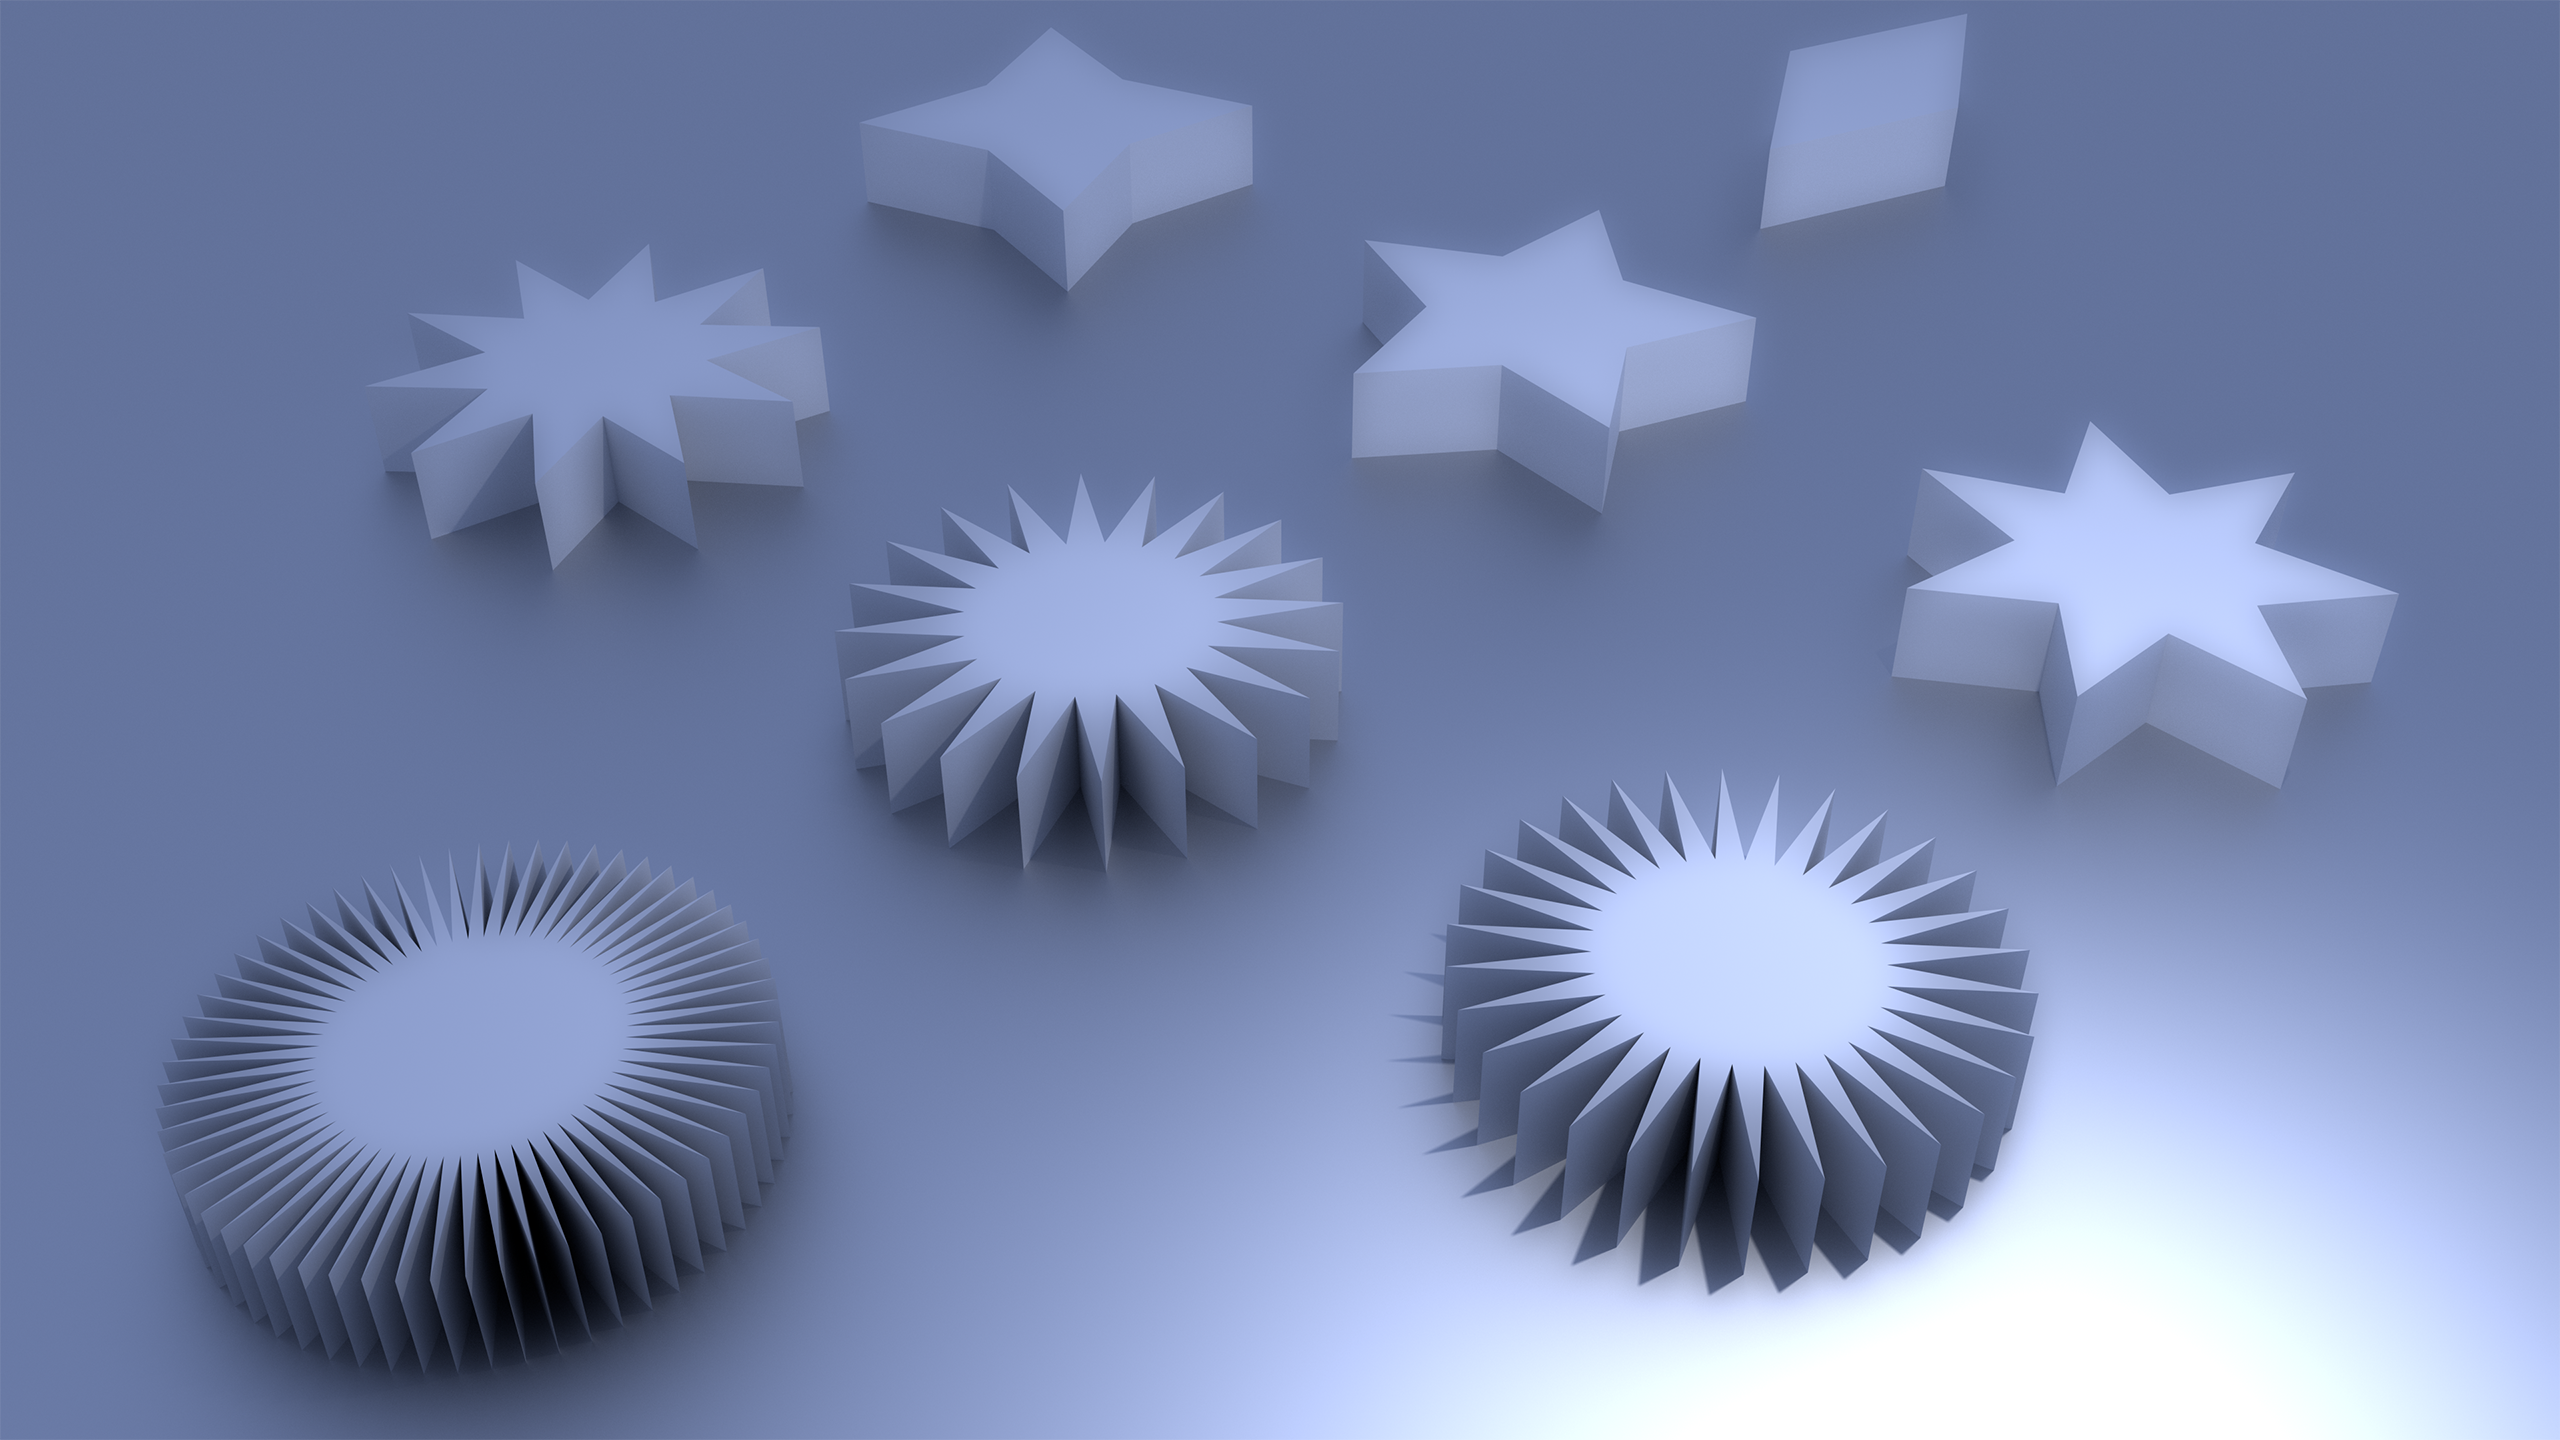
\includegraphics[width=.44\textwidth]{entwurf/star_2-4-5-7-10-20-30-60}}
				{\caption{Gute Unterscheidung von vorn}\label{fig:formen:sterne3d:front}}%
		\end{subfloatrow}
		\hspace*{\columnsep}%
		\begin{subfloatrow}
		\hsize0.7\hsize
		\vbox {%
			\ffigbox[\FBwidth][\FBheight]
				{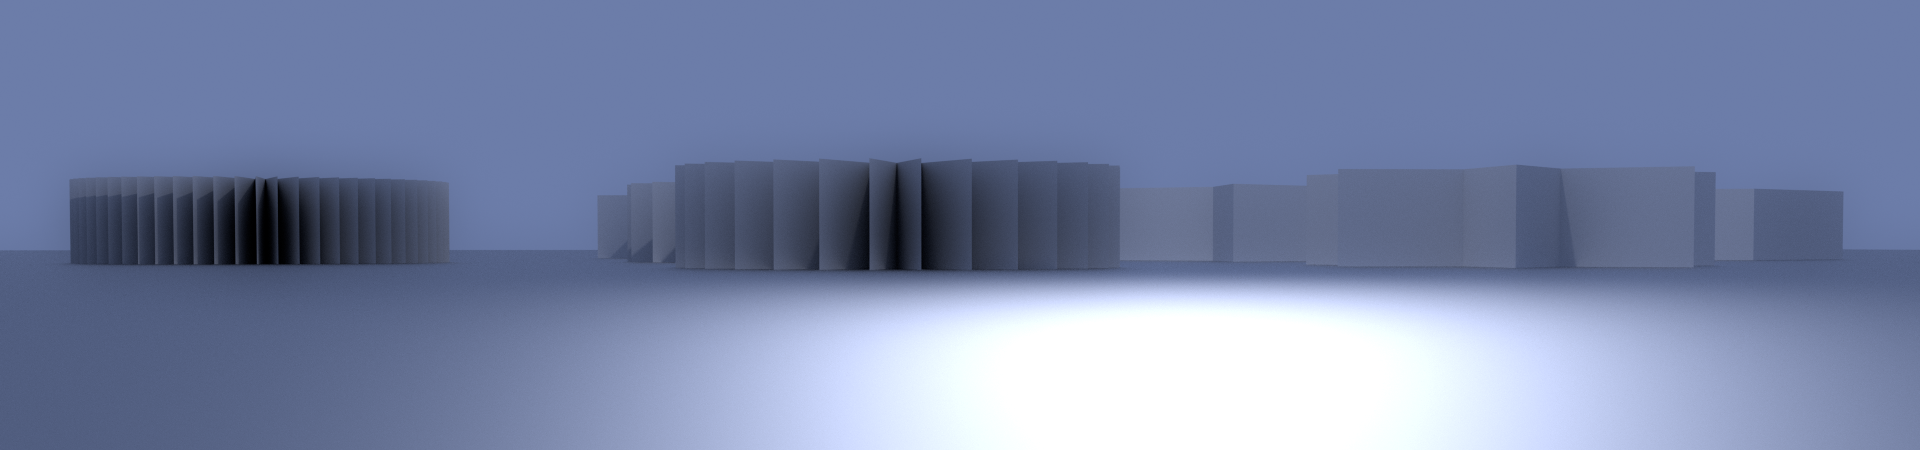
\includegraphics[width=.41\textwidth]{entwurf/star_2-4-5-7-10-20-30-60-seite}}
				{\caption{Die Unterschiede von der Seite \ldots}\label{fig:formen:sterne3d:side}}\vss
			\ffigbox[\FBwidth][\FBheight]
				{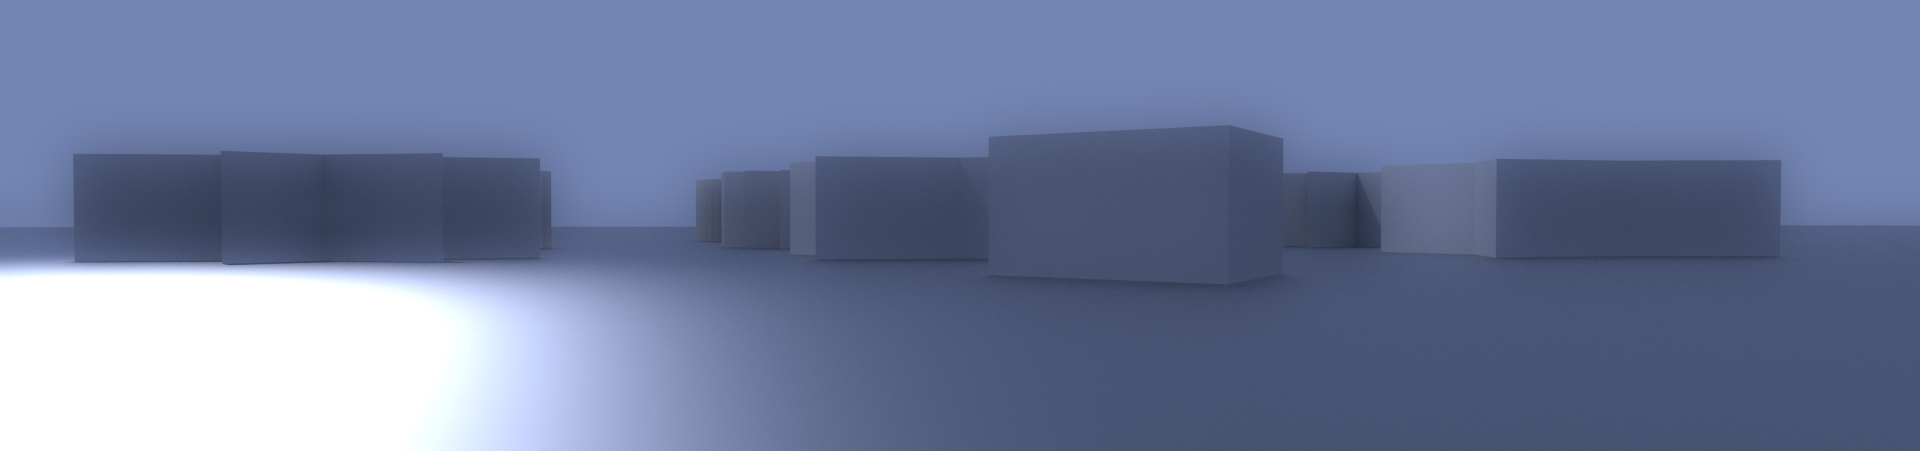
\includegraphics[width=.41\textwidth]{entwurf/star_2-4-5-7-10-20-30-60-oben}}
				{\caption{\ldots bzw. von oben sind kleiner.}\label{fig:formen:sterne3d:top}}
		}
		\end{subfloatrow}
	}
	{\caption{Formgebung mit sternenförmigem, nichtkonvexen Prisma. ERKENNBARKEIT SCHLECHTER ALS BEI TRANS UNTEN?}\label{fig:formen:sterne3d}}
\end{figure}

\begin{figure}
	\ffigbox[\FBwidth] {
		\begin{subfloatrow}
			\ffigbox[\FBwidth][]
			{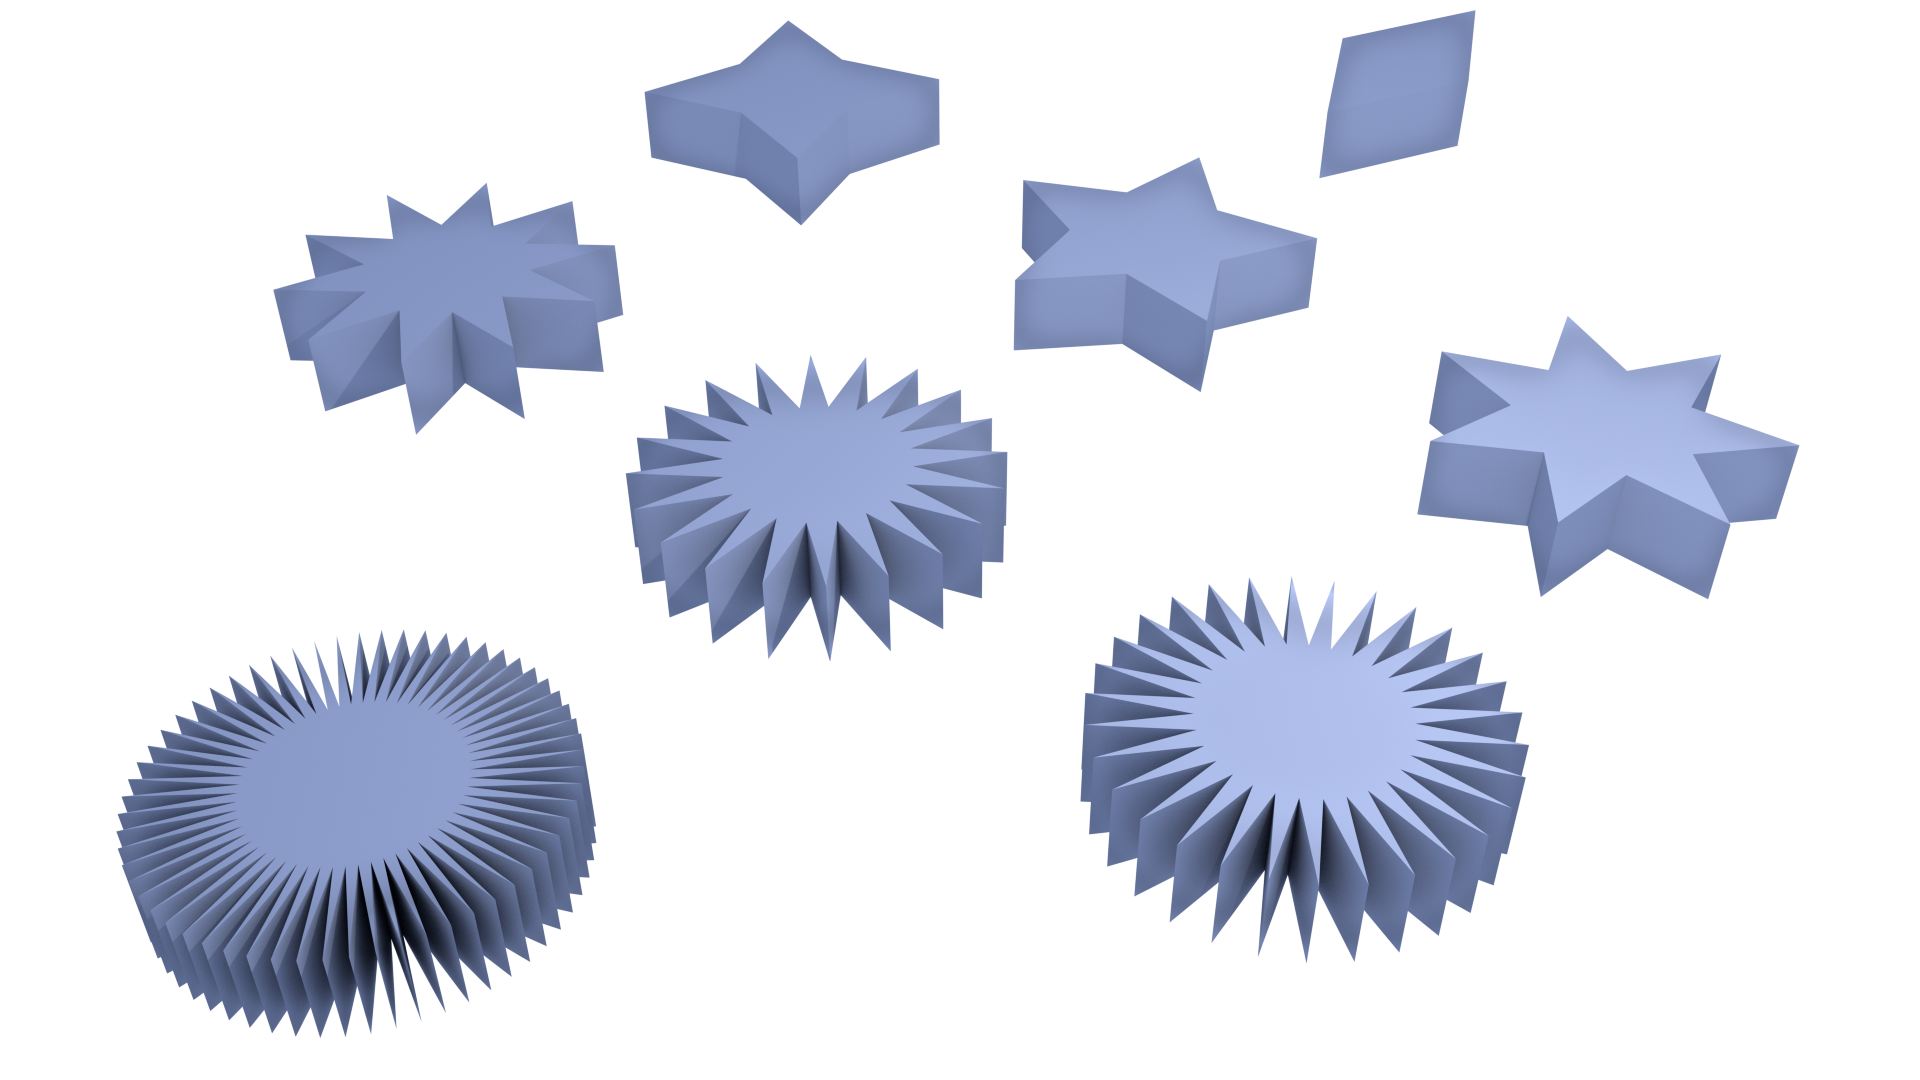
\includegraphics[width=.44\textwidth]{entwurf/star_2-4-5-7-10-20-30-60-trans}}
			{\caption{Gute Unterscheidung von vorn}\label{fig:formen:sterne3d:front-trans}}%
		\end{subfloatrow}
		\hspace*{\columnsep}%
		\begin{subfloatrow}
			\hsize0.7\hsize
			\vbox {%
				\ffigbox[\FBwidth][\FBheight]
				{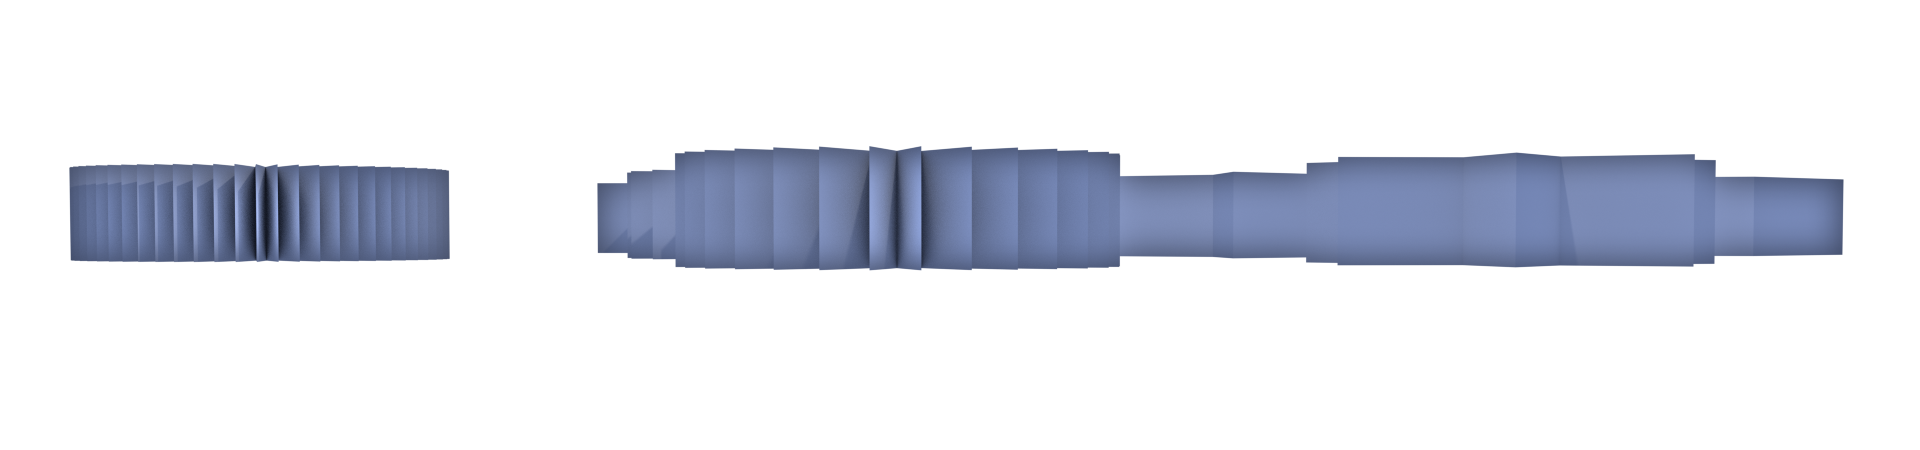
\includegraphics[width=.41\textwidth]{entwurf/star_2-4-5-7-10-20-30-60-seite-trans}}
				{\caption{Die Unterschiede von der Seite \ldots}\label{fig:formen:sterne3d:side-trans}}\vss
				\ffigbox[\FBwidth][\FBheight]
				{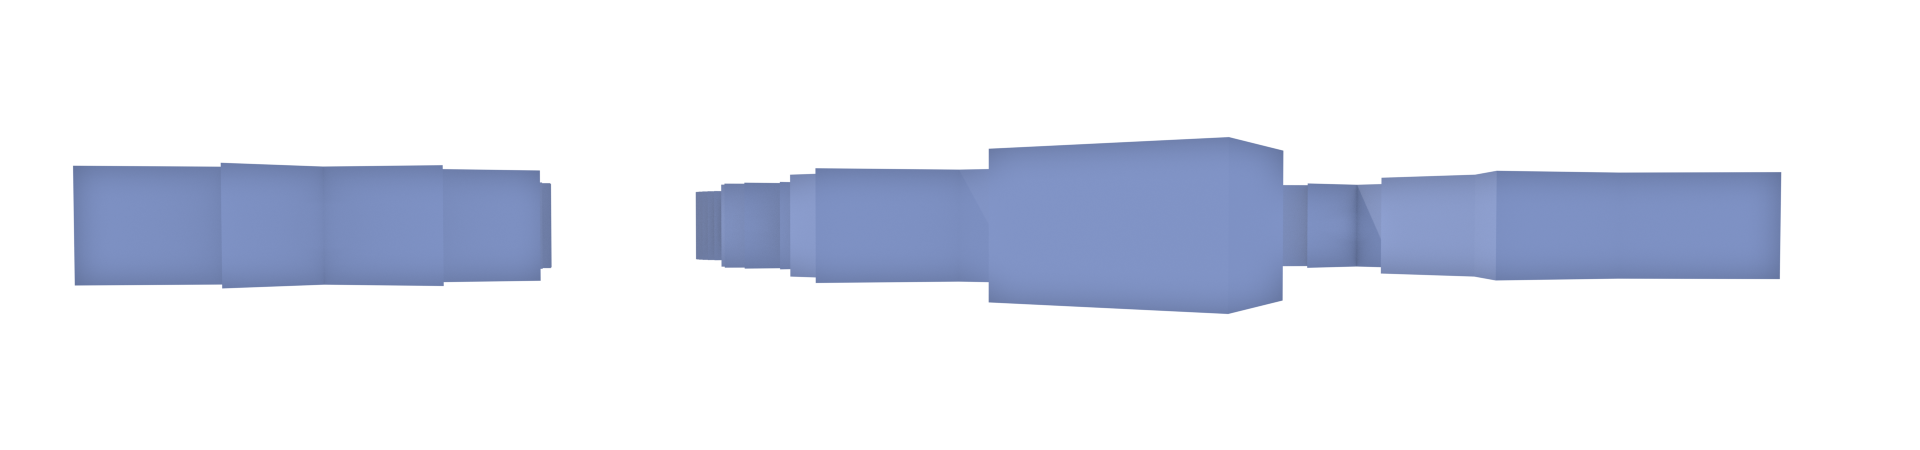
\includegraphics[width=.41\textwidth]{entwurf/star_2-4-5-7-10-20-30-60-oben-trans}}
				{\caption{\ldots bzw. von oben sind kleiner.}\label{fig:formen:sterne3d:top-trans}}
			}
		\end{subfloatrow}
	}
	{\caption{Formgebung mit sternenförmigem, nichtkonvexen Prisma. TRANSPARENT}\label{fig:formen:sterne3d-trans}}
\end{figure}

Die Anforderung, eine Formgebung zu wählen, die einen ähnlichen Umkugelradius und damit eine einheitliche Größe erhält, einen aus allen Winkeln ähnlichen Durchmesser sowie eine ähnliche Form aufweist, führt zu bestimmten Gruppen von Polyedern. Polyeder sind dreidimensionale Polytope und im engeren Sinne eine Teilmenge des \gls{3dRaum}, welche ausschließlich durch gerade Flächen begrenzt wird. Darunter zählen unter anderem die fünf \propernames{platonischen}{platonischer Körper} \cite{RegularPolyhedra}, die 13 \propernames{archimedischen}{archimedischer Körper}, die 13 \propernames{catalanischen}{catalanischer Körper} sowie die 92 \propername{Johnson-Körper} \cite{JohnsonPolyeder}. Eine Charakteristik dieser Polyeder ist ihre konvexe Form, was gleichzeitig die Unterscheidung aus der Distanz erschwert. Die prismatischen Polyeder fallen ebenfalls unter diese Kategorie, werden jedoch aus denselben Gründen ausgeschlossen wie die sternenförmigen Prismen.

Andererseits erfüllen die sternförmigen \propername{Kepler-Poinsot-Körper} (,,Sternpolyeder'') die Anforderungen. Sie besitzen im Gegensatz zu den vorgenannten Polyedern auch konkave Flächen \cite{KeplerPoinsotSolid} und können daher, wie in der interaktiven Visualisierung von \cite{WebGLUniformPolyhedra} zu sehen, leicht von den konvexen Polyedern unterschieden werden.

Ebenfalls geeignet ist der Vorschlag, eine Sternform durch sogenanntes \textquote{Poken} zu erzeugen: \blockcquote[4]{ProceduralGenerationofSculpturalForms}{By “poke” we mean a function to create a pyramid on each face of a given object. (This is different from Kepler’s stellation operation, which extends the face planes.)}

Somit gibt es mit der auf nichtprismatischen Polyedern basierenden Formgebung eine hohe Anzahl verschiedener Formen, die alle die Anforderung an eine einheitliche Größe, an einen aus allen Blickwinkeln ähnlichen Durchmesser und an die Wiedererkennbarkeit gewährleisten. Lediglich die Unterscheidung innerhalb der konvexen Polyeder kann schwerfallen. Am Deutlichsten unterscheiden sich die \propernames{platonischen Körper}{platonischer Körper} untereinander sowie die konvexen von den konkaven, sternförmigen Polyedern.


\section{Visualisierungsentwurf}

\subsection{Taxonomie der Visualisierung}\label{sec:vis-taxonomie}
Die Berechnung des Clusterverhaltens ergibt eine Datenbank, in der Ereignisse abgelegt sind. Ein Ereignis stellt einen Datensatz dieser Datenbank dar, die Parameter des Ereignisses sind die Datensatzfelder. Die Aufgabe der Visualisierung ist es, den Parametern eines Ereignisses visuelle Attribute zuzuweisen. Diese Zuweisung kann in einer weiteren Datenbank als Relation %im Sinne des \gls{rdbms}
zwischen Parameter und Attribut festgehalten werden.

Zum leichteren Verständnis erfolgt eine Einteilung der Parameter, der Attribute sowie der Zuweisungen in die beiden in \autoref{fig:entwurf:taxonomie:vartype} gezeigten Variablentypen. Der Typ \propername{Zahlenwert} steht dabei für die Nutzung eines kontinuierlichen Zahlenraumes, während der Variablentyp \propername{Vokabular} eine diskrete, beschränkte Zuordnung mit voneinander disjunkten Elementen beschreibt.

\begin{figure}
	\begin{tikzpicture}[]
	\node {Variablentyen im Entwurf}
	child { node [value] {Zahlenwert} }
	child { node [vocab] {Vokabular} };
	\end{tikzpicture}
	\caption{Taxonomie der Variablentypen}\label{fig:entwurf:taxonomie:vartype}
\end{figure}

\subsubsection{Parameter eines Ereignisses}
Ein Ereignis besteht aus drei Parametern, die jeweils zwischen ein bis drei Freiheitsgraden aufweisen.

\begin{itemize}
	\item Zeitpunkt: ein Wert (t)
	\item Ort: drei Werte (x, y, z)
	\item Art: ein Vokabular [Split, Merge, Death, Birth]
\end{itemize}

\subsubsection{Visuelle Attribute eines Ereigniselements}\label{sec:attribute}
Die visuellen Attribute können sowohl als fließender \propername{Zahlenwert} als auch als festes \propername{Vokabular} umgesetzt werden. Beispielsweise bedeutet der Vokabulartyp für das \visattrs{Positionsattribut}{Position} die Festlegung bestimmter Koordinaten für jeden Begriff des Vokabulars.

Jedes Attribut besitzt eine individuelle Anzahl an Freiheitsgraden, die zur Visualisierung genutzt werden können.

\begin{itemize}
	\item Position: 3 (x, y, z)
	\item Farbe: 2 (Farbwert/Sättigung, Helligkeit)
	\item Form: 1, eine Wertzuweisung ist möglich durch die Anzahl der Ecken, Kanten und Flächen. Anderes wie z.B. der Abstand der Ecken vom Körperzentrum kollidiert mit dem Attribut Größe.
	\item Größe: 1
	\item Opazität: 1
\end{itemize}

Da Farbwerte bei geringer Sättigung nicht mehr voneinander unterschieden werden können, werden diese beiden Farbeigenschaften zusammengefasst. Dadurch kann die Helligkeit leicht als separates Attribut vom Betrachter erkannt werden, wie in \autoref{fig:entwurf:farbtafel} zu sehen.

\begin{figure}
	VERGLEICHSBILD MIT WECHSELNDER SÄTTIGUNG UND HELLIGKEIT
	%\includegraphics[width=.8\textwidth]{entwurf/}
	\caption{Farbtafel mit unterschiedlicher Sättigung und Helligkeit}\label{fig:entwurf:farbtafel}
\end{figure}

Bei der \visattr{Form} sind mehrere Freiheitsgrade möglich, etwa eine Kombination aus Anzahl der Ecken mit einem variablen Abstand dieser vom Körperzentrum. Der variable Abstand kollidiert jedoch mit dem Attribut \visattr{Größe}. Daher wird das Attribut \visattr{Form} auf einen Freiheitsgrad beschränkt und es werden die in \autoref{sec:grundlagen:formgebung} beschriebenen Polyeder verwendet. Da die Anzahl an Polyedern begrenzt ist und die Unterscheidungsmöglichkeit mit zunehmender Flächenanzahl sinkt, ist das Attribut \visattr{Form} nur eingeschränkt als Zahlenwert verwendbar.

Bei der Bestimmung der Attribute wurde darauf geachtet, ein umfassendes Spektrum der Gestaltgesetze nutzen zu können. Alle visuellen Attribute fallen unter den Einfluss des \viss{Gesetzes der Prägnanz}{Gesetz der Prägnanz}. Mit der \visattr{Position} kann das \vis{Gesetz der Nähe} sowie das \vis{Gesetz der gemeinsamen Region} genutzt werden, eine Kombination aus der \visattr{Position} mit den anderen Attributen resultiert in der Verwendbarkeit des \viss{Gesetzes der Kontinuität}{Gesetz der Kontinuität}. Bis auf die \visattr{Position} kann mit allen visuellen Attributen das \vis{Gesetz der Ähnlichkeit} genutzt werden. Das \vis{Gesetz der Geschlossenheit} kann mit dem \visattrs{Positionsattributs}{Position} verarbeitet werden, falls durch entsprechende Zuweisung die Elemente nah beieinander lägen und sie eine geschlossene Form bilden. Mit den hier definierten Attributen kann somit von sechs der zehn in \autoref{sec:gestaltgesetze} aufgezählten Gestaltgesetze Gebrauch gemacht werden.

Texturen als ein eigenständiges visuelles Attribut werden ausgeklammert, da sie sich mit dem Attribut \visattr{Farbe} und bei der Nutzung als Oberflächenstruktur mit dem Attribut \visattr{Form} überschneiden. Ein Einsatz als Bump Map oder Displacement Map zur Unterstützung des Attributs \visattr{Form} wäre denkbar. Aufgrund dessen, dass bereit Polyeder für das \visattrs{Formattribut}{Form} genutzt werden, wird von einer Verwendung von Texturen allerdings abgesehen.

Animationen bieten weitere visuelle Attribute wie Bewegungsrichtung, Bewegungsbahn, Beschleunigung und Geschwindigkeit als auch die Veränderung der anderen Attribute und eröffnen damit die Nutzung des \viss{Gesetzes der Gleichzeitigkeit}{Gesetz der Gleichzeitigkeit} sowie des \viss{Gesetzes der gemeinsamen Bewegung}{Gesetz der gemeinsamen Bewegung}. Sie werden im Rahmen dieser Arbeit jedoch nicht behandelt.

Die visuellen Attribute lassen sich durch den Betrachter unterschiedlich gut unterscheiden. In der folgenden Sortierung nach ihrer Unterscheidungsgüte stehen die am Leichtesten zu unterscheidenden Attribute ganz oben. (QUELLE)
\begin{enumerate}
	\item Position
	\item Farbwert
	\item Größe
	\item Form
	\item Helligkeit
	\item Opazität
\end{enumerate}

Die Attribute mit höherer Unterscheidungsgüte sollten bevorzugt gewählt werden. Form, Helligkeit und Opazität sind durch die geringere Güte besser als Vokabular- denn als Wertattribut geeignet, da bei den Vokabularen die Anzahl der Begriffe im Vergleich zur Menge der Zahlenwerte gering ist. Dadurch können die Attributseigenschaften weiter auseinanderliegen, was eine leichtere Unterscheidung ermöglicht.

Die 

In der \tool{MegaMol} Molekularsimulation wird ausschließlich das visuelle Attribut \visattr{Position} zur Darstellung genutzt.

\begin{figure}
	\ffigbox[\FBwidth] {
		\begin{subfloatrow}
			\ffigbox[\FBwidth] {
				\fbox {
					\begin{tikzpicture}[level 1/.style={sibling distance=1.4cm}]
					\node {Ereignis}
					child { node [value] {Zeitpunkt} }
					child { node {Ort}
						child [verticalChild, first] { node [value] {x} }
						child [verticalChild, second] { node [value] {y} }
						child [verticalChild, third] { node [value] {z} }
					}
					child { node [vocab] {Art}
						child [verticalChild, first] { node {Split} }
						child [verticalChild, second] { node {Merge} }
						child [verticalChild, third] { node {Death} }
						child [verticalChild, fourth] { node {Birth} }
					};
					\end{tikzpicture}
				}
			}
			{\caption{Ereignis mit Variablentyp}\label{fig:entwurf:taxonomie:ereignis}}%
			
			\ffigbox[\FBwidth] {
				\fbox {
					\begin{tikzpicture}[level 1/.style={sibling distance=1.8cm}]
					\node {Visuelles Attribut}
					child { node {Position}
						child [verticalChild, first] { node [] {x} }
						child [verticalChild, second] { node [] {y} }
						child [verticalChild, third] { node [] {z} }
					}
					child { node {Farbe}
						child [verticalChild, first] { node [] {Farbwert \& S"attigung} }
						child [verticalChild, second] { node [] {Helligkeit} }
					}
					child { node [] {Größe} }
					child { node [] {Form}	}
					child { node [] {Opazität} }
					;
					\end{tikzpicture}
				}
			}
			{\caption{Die visuellen Attribute können beide Variablentypen annehmen.}\label{fig:entwurf:taxonomie:variable}}
		\end{subfloatrow}
	}
	{\caption{Taxonomie der Daten und visuellen Attribute}\label{fig:entwurf:taxonomie}}
\end{figure}

\subsubsection{Problem der lokalen und temporalen Agglomeration}\label{sec:entwurf:agglomeration}

Die Anzahl der Datensätze, die denselben Ort oder denselben Zeitpunkt aufweisen können, ist unbekannt. Schon eine geringe Anzahl identischer Orte oder Zeitpunkte kann je nach Zuordnung der visuellen Attribute zu einer überlagerten, nicht mehr unterscheidbaren Darstellung führen, wodurch die Erkennung solcher Agglomerate nicht gegeben ist. Daher wird ein visuelles Attribut reserviert, um eine solche Anhäufung von Ereignissen anzuzeigen. Die \dataparam{Häufung} wird bei der Zuweisung zu den visuellen Attributen wie ein Ereignisparameter behandelt. Abhängig von dieser Zuweisung in \autoref{sec:entwurf:zuweisung:parameter-attribut} können zwei Werte für die lokale und temporale Häufigkeit notwendig sein. Dieser wird jedem Ereignis zugewiesen und wird beim Auffinden von identischen Ortsparametern bzw. Zeitparametern in den Datensätzen inkrementiert.

Die Begriffe \dataparam{Agglomeration} und \dataparam{Häufung} sind hier synonym.

Bei der Visualisierung von Agglomeraten kann die natürliche Wirkung (QUELLE) der visuellen Attribute genutzt werden. Groß, opaque und dunkel stehen für eine starke Agglomeration. Klein, transparent und hell für eine niedrige.

\subsubsection{Verbundenheit}\label{sec:entwurf:verbundenheit}
Wenn sich ein Cluster teilt (Split) und sich die resultierenden Cluster wiederrum teilen oder mit anderen Clustern verschmelzen (Merge), so kann man diesen Ereignissen Vorgänger (Eltern) sowie Nachfolger (Kinder) zuordnen. IST DAS RICHTIG?

\vis{Gesetz der Geschlossenheit}
\vis{Gesetz der fortgesetzt durchgehenden Linie}
\vis{Gesetz der verbundenen Elemente}


\subsection{Parameter-Attributszuweisung}\label{sec:entwurf:zuweisung:parameter-attribut}

In der \propername{MegalMol} Simulation wird der Ort des Ereignisses mithilfe der Teilchenposition dynamisch visualisiert. Insofern kann angenommen werden, dass für eine nahtlose Benutzbarkeit zwischen der \tool{MegaMol} Animation und der statischen Visualisierung die Zuweisung des Elementattributes \visattr{Position} an den Parameter \dataparam{Ort} empfehlenswert ist. Weiterhin ist die Reservierung der \visattr{Opazität} für die \dataparam{Häufung} die einfachste Möglichkeit, denn dies hat zwei Vorteile. Zum Einen ist keine nachträgliche Modifizierung der visuellen Attribute der einzelnen Ereignisse notwendig, denn die Opazitätseigenschaft sorgt durch Überlagerung für eine von der Anzahl direkt abhängige Hintergrundverdeckung. Dadurch werden zum Anderen auch keine Informationen über die Häufigkeit im Datensatz benötigt. Hingegen muss zum Beispiel eine Größenveränderung nachträglich für jedes Ereignis im Agglomerat auf der Basis eines temporalen oder lokalen \dataparams{Häufungswert}{Häufung} durchgeführt werden.

Darüberhinaus wird jedem Ereignisparameter nur eine visuelles Attribut zugeordnet, denn Mehrfachzuweisungen sollten wegen einer Verminderung der präattentiven Wahrnehmung (VERWEIS AUF GRUNDLAGEN) vermieden werden.

Daraus ergeben sich die in \autoref{tab:entwurf:zuweisung-param-attr:position-agglo} aufgeführten Visualisierungsmöglichkeiten.

\begin{table} 
	\begin{tabularx}{\textwidth}{@{}CCCCCCCCC@{}}
		\toprule
		Attribute & Position x & Position y & Position z & Farbwert \& Sättigung & Helligkeit & Eckenanzahl & Größe & Opazität \tabularnewline
		\midrule
		& Ort x & Ort y & Ort z & Art & Zeit & & & H \tabularnewline
		& Ort x & Ort y & Ort z & Art & & Zeit & & H \tabularnewline 
		& Ort x & Ort y & Ort z & Art & & & Zeit & H \tabularnewline 
		& Ort x & Ort y & Ort z & Art & & & & H \tabularnewline 
		\midrule
		& Ort x & Ort y & Ort z & Zeit & Art & & & H \tabularnewline 
		& Ort x & Ort y & Ort z & & Art & Zeit & & H \tabularnewline
		& Ort x & Ort y & Ort z & & Art & & Zeit & H \tabularnewline 
		& Ort x & Ort y & Ort z & & Art & & & H \tabularnewline 
		\midrule
		& Ort x & Ort y & Ort z & Zeit & & Art & & H \tabularnewline 
		& Ort x & Ort y & Ort z & & Zeit & Art & & H \tabularnewline 
		& Ort x & Ort y & Ort z & & & Art & Zeit & H  \tabularnewline
		& Ort x & Ort y & Ort z & & & Art & & H  \tabularnewline
		\midrule
		& Ort x & Ort y & Ort z & Zeit & & & Art & H \tabularnewline 
		& Ort x & Ort y & Ort z & & Zeit & & Art & H \tabularnewline 
		& Ort x & Ort y & Ort z & & & Zeit & Art & H \tabularnewline 
		& Ort x & Ort y & Ort z & & & & Art & H \tabularnewline 
		\bottomrule
	\end{tabularx}
	\caption{Zuweisungsmöglichkeiten der Parameter zu den visuellen Attributen bei Kopplung des \dataparams{Ortes}{Ort} an die \visattr{Position}. Zur Anzeige der Häufung H wird die \visattr{Opazität} reserviert. Die Zeit wird in einigen Varianten nicht kodiert.}\label{tab:entwurf:zuweisung-param-attr:position-agglo}
\end{table}

Derzeit ist nicht bekannt, wie groß die örtliche Konzentration von Ereignissen ist. Sollte sie eine kritische Anzahl überschreiten und das der \dataparam{Häufung} zugewiesene Attribut keine sinnvollen Ergebnisse mehr liefern können, so kann der Ort des Ereignisses einem anderen Attribut zugewiesen werden. Weiterhin kann das Loslösen des \dataparams{Ortes}{Ort} von der Position sinnvoll sein, wenn für eine Auswertung der Ort des Ereignisses nur eine untergeordnete Rolle spielt. Vorschläge für entsprechende Zuweisungsmöglichkeiten sind in \autoref{tab:entwurf:zuweisung-param-attr:frei} zu finden.

\begin{table}
	\begin{tabularx}{\textwidth}{@{}CCCCCCCCC@{}}
		\toprule
		Attribute & Position x & Position y & Position z & Farbwert \& Sättigung & Helligkeit & Eckenanzahl & Größe & Opazität \tabularnewline
		\midrule
		& Zeit & H & & Art \tabularnewline
		& Zeit & Art & & H & Ort x \tabularnewline
		& Ort x & Art & & & & & H \tabularnewline
		& Ort x & Zeit & & & & H & \tabularnewline
		\bottomrule
	\end{tabularx}
	\caption{Ausgewählte Zuweisungsmöglichkeiten der Parameter zu den visuellen Attributen bei Loslösung des \dataparams{Ortes}{Ort} von der \visattr{Position} sowie Trennung der \dataparam{Häufung} H von der \visattr{Opazität}. Nicht jeder Parameter wird kodiert. UNVOLLSTÄNDIG}\label{tab:entwurf:zuweisung-param-attr:frei}
\end{table}

Da jedoch in der Molekularsimulation der Ort eines Ereignisses der visuellen Position zugewiesen ist und die Visualisierung in der vorliegenden, ersten Iteration mit der Simulation harmonieren soll, erfolgt die Zuweisung des Ortes ausschließlich an die \visattr{Position}, so dass die weitere Betrachtung auf die in \autoref{tab:entwurf:zuweisung-param-attr:position-agglo} gezeigten Zuweisungsmöglichkeiten beschränkt wird.

\subsection{Mockups}\label{sec:mockups}

\subsubsection{Werkzeug}\label{sec:mockups:werkzeug}
Zur Überprüfung einer sinnvollen Zuweisung der Parameter zu den Attributen dienen Mockups. Aufgrund der Vielzahl der in \autoref{sec:entwurf:zuweisung:parameter-attribut} genannten Kombinationsmöglichkeiten wird eine programmatische Erstellung der Mockups gewählt. Da eine schnelle Umsetzbarkeit im Vordergrund steht, wird \propername{Unity3D} als Entwicklungsumgebung gewählt. Ein Vorteil dieser Engine ist die Möglichkeit, rasch Prototypen erstellen zu können sowie die einfache Umsetzbarkeit für verschiedenste Plattformen, ohne auf Containermanager wie \href{https://www.docker.com/}{Docker} angewiesen zu sein. Letzterer Umstand ist für den möglichen Einsatz der Mockups als Evaluationswerkzeug von Bedeutung. Die Performance spielt beim Mockup eine untergeordnete Rolle.

Beim Deploy der \tool{Unity3D} WebGL Anwendung kam es auf bestimmten Apachekonfigurationen zu Problemen. Dies war durch eine \href{http://forum.unity3d.com/threads/html-mem-causes-http-500-internal-server-error-on-apache.309762/}{manuelle Umbenennung von Dateien und Verweisen} in der durch \tool{Unity3D} generierten Anwendung zu lösen. Von offizieller Seite wurde dies \href{http://forum.unity3d.com/threads/html-mem-causes-http-500-internal-server-error-on-apache.309762/#post-2014787}{als Bug markiert}. SOLCHE SÄTZE HABEN IN DER BA VERMUTLICH NIX ZU SUCHEN?

\subsection{Datensatz}\label{sec:mockups:daten}
Um eine Vergleichbarkeit der verschiedenen Mockups zu gewährleisten, liegt ein fester Datensatz in \autoref{tab:entwurf:mockup-data} zugrunde. Sämtliche Werte sind einheitenlos und wurden für die Parameter \dataparam{Ort} und \dataparam{Zeit} so gewählt, dass eine Überlappung der Ereigniselemente von nebeneinanderliegenden Ereignissen bei einer Zuweisung an das visuelle Attribut \visattr{Position} nicht auftritt, da andernfalls durch das \vis{Gesetz der verbundenen Elemente} ein falsches Abbild der zugrundeliegenden Daten übertragen werden würde. Der Zahlenbereich für die Zeit ist auf das Intervall $[1,22]$ begrenzt. Da sich in der Simulation die meisten Elemente mit zunehmender Zeit vom Zentrum entfernen, wird die $x$-Koordinate des Ortes mit \autoref{eq:mockup:zeit-ortx} direkt an die Zeit $t$ gekoppelt.
\begin{align}\label{eq:mockup:zeit-ortx}
	x = \left\lfloor\frac 43\cdot t + 0,5\right\rfloor
\end{align}
Aufgrund des zylinderförmigen Raumes in der Simulation wird sowohl für die $y$-Koordinate als auch für die $z$-Koordinate des Ortes ein identisches und kleineres Intervall von $[1,10]$ gewählt.

Die Zuweisung der \dataparam{Art} des Ereignisses erfolgt manuell. Da die simulierten Partikel in der \tool{MegaMol} zu Beginn der Simulation einen einzigen Cluster in flüssiger Phase bilden, kommen bei kleinen Zeitwerten vor allem Splits vor.

Zur Darstellung der in \autoref{sec:entwurf:agglomeration} beschriebenen Häufung, werden die Ereignisse $6-9$, $35/36$ sowie $46-48$ jeweils gruppiert und händisch an denselben Ort und dieselbe Zeit gesetzt.


\subsubsection{Zuweisung der Zahlenwerte}
Zur Gewährleistung der in \autoref{sec:mockups:daten} beschriebenen Vermeidung unnötiger Überlappungen der Ereigniselemente wird der Standardwert des Attributs \visattr{Größe}, d.h. wenn das Attribut keinem Parameter zugewiesen ist, entsprechend skaliert. Um nah bei der Visualisierung der Molekularsimulation selbst zu bleiben, wird in den Mockups, die nicht das Attribut \visattr{Form} beinhalten, eine Kugel verwendet. 

Die Attribute in den Mockups weisen folgende Zahlenbereiche auf:
\begin{itemize}
	\item x-, y-, z-Position: $[-\infty, \infty]$, beim Parameter \dataparam{Ort} erfolgt eine direkte Zuweisung 
	\item Farbwert: $[0, 340]\degree$ bei $100\%$ Sättigung (\gls{hsb} Modell)
	\item Helligkeit $[40, 100]\%$, Standardwert $100\%$ (\gls{hsb}-Modell)
	\item Form: besitzt keinen Zahlenbereich, sondern beinhaltet verschiedene Formen von Polyedern sowie die Kugel als Standardwert
	\item Skalierung: $[0.25,2]$, Standardwert $1$
	\item Opazität: $[40, 100]\%$, Standardwert $100\%$
\end{itemize}
Die Mindesthelligkeit $b_{\text{min}}$ von $40\%$ dient dazu, um noch eine Farbwertunterscheidung treffen zu können, genauso wie die Mindestopazität von ebenfalls $40\%$. Der Maximalfarbwert $h_{\text{max}}$ von $340\degree$ wird festgelegt, um eine Unterscheidung zu den niedrigen Farbwerten zu erhalten.

Da die Grenzwerte der visuellen Attribute $a_{\text{min}}$ und $a_{\text{max}}$ aus \autoref{sec:mockups} bekannt sind und sich für die Parameter $p$ aus \autoref{tab:entwurf:mockup-data} ein minimaler und maximaler Wert $p_{\text{min}}$ und $p_{\text{max}}$ bestimmen lässt, wird für die Berechnung der Attributwerte die Linearfunktion in \autoref{eq:mockup-linearfunktion} verwendet.

\begin{equation}
\begin{aligned}\label{eq:mockup-linearfunktion}
a &= m \cdot p + n\\
a_{\text{max}} &= m \cdot p_{\text{max}} + n\\
a_{\text{min}} &= m \cdot p_{\text{min}} + n\\
m &= \boxed{\frac{a_{\text{max}} - n}{p_{\text{max}}}}\\
n &= a_{\text{min}} - m \cdot {p_{\text{min}}} = a_{\text{min}} - \frac{a_{\text{max}} - n}{p_{\text{max}}} \cdot p_{\text{min}}\\
&= a_{\text{min}} - a_{\text{max}} \cdot \frac {p_{\text{min}}}{p_{\text{max}}} + n \cdot \frac {p_{\text{min}}}{p_{\text{max}}}\\
n \cdot p_{\text{max}} &= a_{\text{min}} \cdot p_{\text{max}} - a_{\text{max}} \cdot p_{\text{min}} + n \cdot p_{\text{min}}\\
n \cdot \left( p_{\text{max}} - p_{\text{min}}\right) &= a_{\text{min}} \cdot p_{\text{max}} - a_{\text{max}} \cdot p_{\text{min}}\\
n &= \boxed{\frac{a_{\text{min}} \cdot p_{\text{max}} - a_{\text{max}} \cdot p_{\text{min}}}{p_{\text{max}} - p_{\text{min}}}}\\
\end{aligned}
\end{equation}

Anschließend erfolgt eine Rundung zur handlichen Verwendung der Ergebnisse.
\begin{align}\label{eq:mockup-rundung}
	a = \left\lfloor m \cdot p + n + 0,5 \right\rfloor
\end{align}

Die Berechnungsergebnisse sind in \autoref{sec:mockups:berechnungen} zu finden.

\subsubsection{Zuweisung des Vokabulars}

Da die Mächtigkeit $M$ des Vokabulars von \dataparam{Art} bekannt ist, kann das Intervall $v$ des Attributs $a$ in \autoref{eq:mockup-vokabular} zur rechnerischen Ermittlung der Attributwerte $a_i$ genutzt werden.

\begin{equation}
\begin{aligned}\label{eq:mockup-vokabular}
M &= 4\\
\Rightarrow p_{0\ldots 3} &= \left( 0, \frac 13, \frac 23, 1 \right) \\
v &= a_{\text{max}} - a_{\text{min}}\\
\\
a_i &= \left\lbrace p_i \cdot v + a_{\text{min}} \left| 0 \le i \le M-1 \right. \right\rbrace 
\end{aligned}
\end{equation}

Ausnahmen bilden die Attribute \visattr{Farbe} und \visattr{Form}. Wegen der kleinen Mächtigkeit des Vokabulars und zur Sicherung einer optimale Aufteilung des Farbwerts, wird dieser in \autoref{tab:entwurf:mockup-art} manuell definiert. Bei dem Attribut \visattr{Form} werden zur optimalen Unterscheidung vier Varianten aus der Menge der \propernames{platonischen Körper}{platonischer Körper} ausgewählt.

\begin{table}
	\begin{tabularx}{\textwidth}{@{}CRRRCR@{}}
		\toprule
		Art & Farbwert [°] & Helligkeit [\%] & Position x & Form & Größe \tabularnewline
		\midrule
		Death & 0   & 40  & 1  & T & 0,25 \tabularnewline
		Merge & 55  & 60  & 11 & H & 0,83 \tabularnewline
		Split & 245 & 80  & 21 & O & 1,42 \tabularnewline
		Birth & 145 & 100 & 31 & D & 2 \tabularnewline
		\bottomrule
	\end{tabularx}
	\caption{Festlegung der Attributeigenschaften für den Parameter \dataparam{Art} in den Mockups.}\label{tab:entwurf:mockup-art}
\end{table}

\subsubsection{Ausnahme: Konstanter Attributswert bei Opazität}

Aus den in \autoref{sec:entwurf:zuweisung:parameter-attribut} aufgeführten Gründen ist es sinnvoll, die \visattr{Opazität} der \dataparam{Häufung} zuzuweisen und sie mit einem konstanten Variablentyp auszustatten, so dass keine zusätzliche Ereigniswerte für die \dataparam{Agglomeration} benötigt werden. Dieser konstante Wert wird auf $50\%$ Opazität festgesetzt.

\subsection{Unterscheidbarkeit von Polyedern}

Da die Unterscheidung von Polyedern mit zunehmender Flächenanzahl schwieriger wird, findet im Mockup eine Begrenzung auf die fünf \propernames{platonischen Körper}{platonischer Körper} mit einer geringen Ecken- und Flächenanzahl statt.
\begin{description}
	\item[T] Tetraeder mit 4 Ecken und 4 Flächen
	\item[O] Oktaeder mit 6 Ecken und 8 Flächen
	\item[H] Hexaeder mit 8 Ecken und 6 Flächen
	\item[I] Icosaeder mit 12 Ecken und 20 Flächen
	\item[D] Dodekaeder mit 20 Ecken und 12 Flächen
\end{description}
Die Abkürzungen folgen dem Vorschlag von Baierl \cite[S.~42]{KonvexePolyeder}. Bei der Modellierung in \tool{Blender} wurde für die Meshes die maximale Dimension von $1$ (einheitenlos) entsprechend der Dimension der kugelförmigen Standardelemente in \tool{Unity3D} gewählt.


\section{Entwurfsauswertung}

In den Abbildungen \autoref{fig:entwurf:frei} sind Beispiele dafür zu sehen, wenn die \dataparam{Häufung} anderen Attributen außer der \visattr{Opazität} zugewiesen wird.

\begin{figure}
	\caption{Mockups mit freier Positionszuweisung.}\label{fig:entwurf:frei}
\end{figure}

\subsection{Glyphen}
- Polygone nicht so gut geeignet, da Unterscheidung auf Entfernung schwer möglich und auch hier noch Abhängigkeit vom Blickwinkel
- daher zweidimensionale, vordefinierte Bilder an Eventtypen gekoppelt, immer zur Kamera ausgerichtet vgl. Sprites

Hier viel aus den Grundlagen Entwurfsabschnitten mit reinnehmen inkl. 3D-Prototyp!

\section{Vorgehen}
\subsection{Gestaltung der Glyphen}
\subsection{Renderer}
Shader:
common.btf für Standardlicht
billboard.btf für Billboards in OGL 2.1
Nutzung von OpenGL 2.1 zur Wahrung der Kompatibilität mit den MM Modulen.
Laden der Bilder mit lodepng

Nutzung der glm Bibliothek, da dadurch die Datentypen in C++ und in GLSL konsistent angelegt werden können.

\subsection{Weiterleitung der Daten}

Wie werden die Variablen im Call gefüllt bzw. die Funktionen zum Füllen aufgerufen? Gefüllt werden sie entweder durch den Calculator oder die Source. Verwendung von Zeigern, um keine Daten wiederholt zu kopieren.


\chapter{Evaluation}

Diskussion: was funktioniert/nicht

keine Bestimmung der Güte der Heuristik bei der Ereigniserkennung

Zeit- und Ressourcenangaben beziehen sich auf folgendes System:
- Intel Core i5-3210M
- 2x4GB DDR3-1600
- Windows 8.1

Zeitmessung in C++: http://stackoverflow.com/a/21995693

Variablentyp um Loops zu zählen:
mit size\_t anstatt von int:
Die Idee von size\_t ist, (1) dass man vielleicht eine Obergrenze hat, die ein size\_t ist, und sich so den Cast im Vergleich spart, damit der Compiler nicht warnt
[15:36:44] Max: Und (2) dass es im Allgemeinen so groß wie ein Register der CPU ist
Nur dass (2) trotzdem nicht so clever ist, weil ich mal ohne Quelle behaupte, dass 32-Bit-Operationen auf 64-Bit-CPUs genauso schnell wie 64-Bit-Operationen, und im Zweifelsfalle sogar schneller sind
[15:37:25] Max: (Weil die Instruktionen kürzer sind)
[15:37:42 | Bearbeitet 15:37:43] Max: Also mit 64-Bit-CPUs meine ich x64
Und „wie du oben sagtest“: Nein, ich meinte, weil 8-Bit-Operationen wiederum im Zweifel langsamer sind als einfache Operationen auf int
[15:38:39] Max: Auch für int8\_t würde das gelten
[15:38:46] Max: Bei x86 nicht, aber bei ARM bestimmt, beispielsweise


\chapter{Zusammenfassung}
Kurzzusammenfassung/Abstract ausführlicher, auf Details eingehen

\chapter{Ausblick}
Verbesserung des Algorithmus:
\begin{itemize}
	\item Einbeziehung von sowohl der Forward- als auch der Backwardsliste bei der Ermittlung von Merge und Split.
	\item Vergleich von Clustern über mehrere Zeitschritte. Dazu eine Signatur für jeden Cluster nutzen, die beispielsweise mit der Summe der Partikelidentifikatoren gebildet werden kann.
	\item Nutzung der Nachbarschaften von Clustern, wie mit dem Nachbarschaftsgraphen vorgeschlagen
	\item MMSE Datenformat: Eventeinteilung nach Typ oder Zeit (weniger Speicherplatz)
\end{itemize}

Weitere Untersuchungsmöglichkeiten der Visualisierung:
\begin{itemize}
	\item Nutzung von Animationen mit visuellen Bewegungsattributen (Bewegungsrichtung, Bewegungsbahn, Beschleunigung, Geschwindigkeit) sowie Veränderung der anderen Attribute; die Zuweisung der Bewegungsattribute wäre an die Parameter Zeit und Position denkbar, die Zuweisung der Veränderung der anderen Attribute kann an alle drei Parameter erfolgen
	\item Attribut \visattr{Position} als \propername{Vokabular} bei örtlicher Häufung von Ereignissen
	\item Wirkung der Farbzuordnung untersuchen
	\item Elementattribute (Größe, Opazität) abhängig vom Zoom
%	\item \visattr{Form}: Polyeder on-the-fly berechnen für unendlich viele Varianten (bei konvexen: vertex [0f-2f] und edge truncation [0f-1f], siehe Blender/Regular Solids) und offene Formen erlauben (keine Flächen, nur dicke Kanten), vgl. \cite{WebGLUniformPolyhedra}.
\end{itemize}

Benutzung von flexiblen Isooberflächen nach \cite{carr2010flexibleIsosurfaces}.



\appendix

\chapter{Anhang}

\section{Berechnungen Mockups}\label{sec:mockups:berechnungen}

\begin{table} 
	\begin{tabularx}{\textwidth}{@{}RRRC@{}}
		\toprule
		Datensatznummer & Zeitpunkt $t$ & Ort ($x, y, z$) & Art \tabularnewline
		\midrule
1	   &   	1	   &   	$1	   ,	8	   ,	4$	   &   	Split \tabularnewline
2	   &   	1	   &   	$1	   ,	4	   ,	3$	   &   	Split \tabularnewline
3	   &   	1	   &   	$1	   ,	1	   ,	8$	   &   	Split \tabularnewline
4	   &   	1	   &   	$1	   ,	4	   ,	1$	   &   	Split \tabularnewline
5	   &   	1	   &   	$1	   ,	4	   ,	9$	   &   	Split \tabularnewline
6	   &   	1	   &   	$1	   ,	4	   ,	4$	   &   	Split \tabularnewline
7	   &   	1	   &   	$1	   ,	4	   ,	4$	   &   	Merge \tabularnewline
8	   &   	1	   &   	$1	   ,	4	   ,	4$	   &   	Birth \tabularnewline
9	   &   	1	   &   	$1	   ,	4	   ,	4$	   &   	Death \tabularnewline
10	   &   	1	   &   	$1	  , 	4	  , 	6$	   &   	Split \tabularnewline
11	   &   	2	   &   	$3	  , 	4	  , 	1$	   &   	Split \tabularnewline
12	   &   	2	   &   	$3	  , 	8	  , 	7$	   &   	Birth \tabularnewline
13	   &   	2	   &   	$3	  , 	7	  , 	8$	   &   	Split \tabularnewline
14	   &   	2	   &   	$3	  , 	6	  , 	1$	   &   	Split \tabularnewline
15	   &   	2	   &   	$3	  , 	1	  , 	2$	   &   	Merge \tabularnewline
16	   &   	2	   &   	$3	  , 	5	  , 	8$	   &   	Split \tabularnewline
17	   &   	3	   &   	$4	  , 	3	  , 	1$	   &   	Merge \tabularnewline
18	   &   	3	   &   	$4	  , 	10	 ,  	10$	   &   	Merge \tabularnewline
19	   &   	3	   &   	$4	  , 	5	  , 	4$	   &   	Merge \tabularnewline
20	   &   	3	   &   	$4	  , 	3	  , 	1$	   &   	Merge \tabularnewline
21	   &   	4	   &   	$5	  , 	5	  , 	7$	   &   	Merge \tabularnewline
22	   &   	4	   &   	$5	  , 	3	  , 	1$	   &   	Split \tabularnewline
23	   &   	4	   &   	$5	  , 	3	  , 	10$	   &   	Merge \tabularnewline
24	   &   	4	   &   	$5	  , 	1	  , 	1$	   &   	Split \tabularnewline
25	   &   	5	   &   	$7	  , 	9	  , 	1$	   &   	Merge \tabularnewline
26	   &   	5	   &   	$7	  , 	4	  , 	2$	   &   	Merge \tabularnewline
27	   &   	6	   &   	$8	  , 	3	  , 	9$	   &   	Split \tabularnewline
28	   &   	6	   &   	$8	  , 	10	 ,  	10$	   &   	Death \tabularnewline
29	   &   	6	   &   	$8	  , 	1	  , 	5$	   &   	Split \tabularnewline
30	   &   	6	   &   	$8	  , 	8	  , 	1$	   &   	Death \tabularnewline
31	   &   	7	   &   	$9	  , 	3	  , 	5$	   &   	Death \tabularnewline
32	   &   	7	   &   	$9	  , 	6	  , 	4$	   &   	Death \tabularnewline
33	   &   	8	   &   	$11	 ,  	3	 ,  	8$	   &   	Split \tabularnewline
34	   &   	8	   &   	$11	 ,  	3	 ,  	2$	   &   	Split \tabularnewline
35	   &   	10	   &   	$13	,   	2	,   	7$	   &   	Merge \tabularnewline
36	   &   	10	   &   	$13	,   	2	,   	7$	   &   	Split \tabularnewline
37	   &   	10	   &   	$13	,   	10	,	   	5$	   &   	Merge \tabularnewline
38	   &   	10	   &   	$13	,   	2	,   	2$	   &   	Split \tabularnewline
39	   &   	13	   &   	$17	,   	8	,   	1$	   &   	Merge \tabularnewline
40	   &   	13	   &   	$17	,   	1	,   	8$	   &   	Merge \tabularnewline
41	   &   	15	   &   	$20	,   	5	,   	3$	   &   	Split \tabularnewline
42	   &   	15	   &   	$20	,   	7	,   	6$	   &   	Split \tabularnewline
43	   &   	16	   &   	$21	,   	7	,   	3$	   &   	Death \tabularnewline
44	   &   	16	   &   	$21	,   	6	,   	6$	   &   	Merge \tabularnewline
45	   &   	18	   &   	$24	,   	8	,   	4$	   &   	Merge \tabularnewline
46	   &   	20	   &   	$27	,   	6	,   	5$	   &   	Merge \tabularnewline
47	   &   	20	   &   	$27	,   	6	,   	5$	   &   	Merge \tabularnewline
48	   &   	20	   &   	$27	,   	6	,   	5$	   &   	Death \tabularnewline
49	   &   	21	   &   	$28	,   	5	,   	4$	   &   	Merge \tabularnewline
50	   &   	21	   &   	$28	,   	5	,   	3$	   &   	Merge \tabularnewline
		\bottomrule
	\end{tabularx}
	\caption{Die Beispieldatensätze für die Mockups. Die $x$-Koordinate des Ortes ist mit dem Zeitpunkt $t$ gekoppelt über $x=\left\lfloor\frac 43\cdot t + 0,5\right\rfloor$. Die $y,z$-Koordinaten sind, bis auf wenige Ausnahmen zur Demonstration der Häufung, zufällig verteilt im Intervall $[1, 10]$.}\label{tab:entwurf:mockup-data}
\end{table}

WERTE VERALTET BZW. ZEIGEN DER TRIVIALEN BERECHNUNG SINNLOS/KANN GELÖSCHT WERDEN

In \autoref{eq:mockup-zeit-farbwert} ist die Berechnung des Farbwerts $h$ in linearer Abhängigkeit von der Zeit $t$ zu finden.
\begin{equation}
\begin{aligned}\label{eq:mockup-zeit-farbwert}
h [\degree] &= m \cdot t + n\\
h_{\text{max}} &= m \cdot t_{\text{max}} + n &\text{mit } h_{\text{max}} = 320, t_{\text{max}} = 23\\
h_{\text{min}} &= m \cdot t_{\text{min}} + n &\text{mit } h_{\text{min}} = 0, t_{\text{min}} = 1\\
n &= -14,\overline{54}\\
m &= 14,\overline{54}\\
h [\degree] &= \boxed{\left\lfloor  14,\overline{54} \cdot t + 14,\overline{54} + 0,5 \right\rfloor}
\end{aligned}
\end{equation}

In \autoref{eq:mockup-zeit-helligkeit} wird die Berechnung der Helligkeit $b$ in linearer Abhängigkeit von der Zeit $t$ gezeigt.
\begin{equation}
\begin{aligned}\label{eq:mockup-zeit-helligkeit}
	b [\%] &= m \cdot t + n\\
	b_{\text{max}} &= m \cdot t_{\text{max}} + n &\text{mit } b_{\text{max}} = 100, t_{\text{max}} = 23\\
	b_{\text{min}} &= m \cdot t_{\text{min}} + n &\text{mit } b_{\text{min}} = 40, t_{\text{min}} = 1\\
	n &= 37,\overline{27}\\
	m &= 2,\overline{72}\\
	b [\%] &= \boxed{\left\lfloor 2,\overline{72} \cdot t + 37,\overline{27} + 0,5 \right\rfloor}
\end{aligned}
\end{equation}

In \autoref{eq:mockup-zeit-durchmesser} ist die Berechnung der Durchmesser $d$ in linearer Abhängigkeit von der Zeit $t$ zu finden.
\begin{equation}
\begin{aligned}\label{eq:mockup-zeit-durchmesser}
	d [\text{px}] &= m \cdot t + n\\
	d_{\text{max}} &= m \cdot t_{\text{max}} + n &\text{mit } d_{\text{max}} = 75, t_{\text{max}} = 23\\
	d_{\text{min}} &= m \cdot t_{\text{min}} + n &\text{mit } d_{\text{min}} = 25, t_{\text{min}} = 1\\
	n &= 22,\overline{72}\\
	m &= 2,\overline{27}\\
	d [\text{px}] &= \boxed{\left\lfloor 2,\overline{27} \cdot t + 22,\overline{72} + 0,5 \right\rfloor}
\end{aligned}
\end{equation}

Analog erfolgen die Berechnungen für den Parameter \dataparam{Ort} x mit den Grenzwerten
\begin{equation}
\begin{aligned}\label{eq:mockup-ortx-grenzwerte}
	x_{\text{min}} &= 1\\
	x_{\text{max}} &= 31
\end{aligned}
\end{equation}
Das Ergebnis ist in \autoref{tab:entwurf:mockup-ortx} zu finden.

\begin{table}
	\begin{tabularx}{\textwidth}{@{}RRRRR@{}}
		\toprule
		Zeit & Farbwert [°] & Helligkeit [\%] & Anzahl Ecken & Größe [px] \tabularnewline
		\midrule
		 1 & 0 & 40 & 1 & 25 \tabularnewline
		 2 & 15 & 43 & 2 & 27 \tabularnewline
		 3 & 29 & 45 & 3 & 30 \tabularnewline
		 4 & 44 & 48 & 4 & 32 \tabularnewline
		 5 & 58 & 51 & 5 & 34 \tabularnewline
		 6 & 73 & 54 & 6 & 36 \tabularnewline
		 7 & 87 & 56 & 7 & 39 \tabularnewline
		 8 & 102 & 59 & 8 & 41 \tabularnewline
		 10 & 131 & 65 & 10 & 45 \tabularnewline
		 13 & 175 & 73 & 13 & 52 \tabularnewline
		 15 & 204 & 78 & 15 & 57 \tabularnewline
		 16 & 218 & 81 & 16 & 59 \tabularnewline
		 20 & 276 & 92 & 20 & 68 \tabularnewline
		 21 & 291 & 95 & 21 & 70 \tabularnewline
		 23 & 320 & 100 & 23 & 75 \tabularnewline
		\bottomrule
	\end{tabularx}
	\caption{Festlegung der Attributeigenschaften für den Parameter \dataparam{Zeit} in den Mockups. VERALTET}\label{tab:entwurf:mockup-zeit}
\end{table}


\begin{table}
	\begin{tabularx}{\textwidth}{@{}RRRRR@{}}
		\toprule
		Ort x & Farbwert [°] & Helligkeit [\%] & Anzahl Ecken & Größe [px] \tabularnewline
		\midrule
		1 & 0 & 40 & 1 & 25 \tabularnewline
		3 & 21 & 44 & 3 & 28 \tabularnewline
		4 & 32 & 46 & 4 & 30 \tabularnewline
		5 & 43 & 48 & 5 & 32 \tabularnewline
		7 & 64 & 52 & 7 & 35 \tabularnewline
		8 & 75 & 54 & 8 & 37 \tabularnewline
		9 & 85 & 56 & 9 & 38 \tabularnewline
		11 & 107 & 60 & 11 & 42 \tabularnewline
		13 & 128 & 64 & 13 & 45 \tabularnewline
		17 & 171 & 72 & 17 & 52 \tabularnewline
		20 & 203 & 78 & 20 & 57 \tabularnewline
		21 & 213 & 80 & 21 & 58 \tabularnewline
		27 & 277 & 92 & 27 & 68 \tabularnewline
		28 & 288 & 94 & 28 & 70 \tabularnewline
		31 & 320 & 100 & 31 & 75 \tabularnewline
		\bottomrule
	\end{tabularx}
	\caption{Festlegung der Attributeigenschaften für den Parameter \dataparam{Ort} x in den Mockups. VERALTET}\label{tab:entwurf:mockup-ortx}
\end{table}


\section{Werkzeuge und Bibliotheken}\label{sec:anhang:werkzeuge}

\subsubsection{Mockup Visualisierung}
\begin{description}
	\item [Adobe Illustrator]
	\item [Blender] mit Regular Solids
	\item [Unity3D] mit \href{http://forum.unity3d.com/threads/a-working-stylable-combo-box-drop-down-list.264167/}{UIComboBox}, \href{http://forum.unity3d.com/threads/fly-cam-simple-cam-script.67042/}{Simple FlyCamera} 
\end{description}

\subsubsection{Dokumentation}
\begin{description}
	\item [Adobe Photoshop]
	\item [Blender] mit Extra Objects
	\item [TeXstudio, TeXlive] mit tudscr, glossaries, tikz u.a.
\end{description}

\subsubsection{MegaMol Plugin}
\begin{description}
	\item [ActivePerl]
	\item [glm]
	\item [lodepng] zum Laden von Texturen
	\item [MegaMol] mit ANN, AntTweakBar, mmstd\_datatools, vislib
	\item [MegaMolConf]
	\item [VisualStudio 2013] mit OpenMP
\end{description}

%\backmatter %Nachspann: Römische Seitennummerierung

\printbibliography[heading=bibintoc]\label{sec:bibliography}

\printindex % Überschriftentyp in \indexsetup, level

\end{document}